% !TEX encoding = IsoLatin2  % notwendige Zeile f"ur Mac-Benutzer (muss als Kommentar stehen); Windows-Benutzer k"onnen die Zeile l"oschen.

% LaTeX-Vorlage Version 3.1,  Juli 2011
% erstellt von Dr. Andreas Drauschke (andreas.drauschke@technikum-wien.at) und Dr. Susanne Teschl (susanne.teschl@technikum-wien.at)
% geringf"ugig adaptiert von Harald Stockinger (harald.stockinger@technikum-wien.at)

 
\documentclass[a4paper,bibtotoc,oneside]{scrbook} 
% F"ur kurze Arbeiten w"are auch die Dokumentklasse "scrartcl" ausreichend. In diesem Fall ist "section" die h"ochste Ebene ("chapter" gibt es dann nicht).
% \documentclass[a4paper,bibtotoc,oneside]{scrartcl}


% verlinkte Querverweise im pdf
\usepackage{hyperref}

% deutsche Anpassungen
\usepackage[utf8]{inputenc}
\usepackage[T1]{fontenc}
\usepackage[ngerman]{babel}

% mathematische Symbole
\usepackage{amsmath,amssymb,amsfonts,amstext}

% Kopfzeilen frei gestaltbar
\usepackage{fancyhdr}
\lfoot[\fancyplain{}{}]{\fancyplain{}{}}
\rfoot[\fancyplain{}{}]{\fancyplain{}{}}
\cfoot[\fancyplain{}{\footnotesize\thepage}]{\fancyplain{}{\footnotesize\thepage}}
\lhead[\fancyplain{}{\footnotesize\nouppercase\leftmark}]{\fancyplain{}{}}
\chead{}
\rhead[\fancyplain{}{}]{\fancyplain{}{\footnotesize\nouppercase\sc\leftmark}} 

% Farben im Dokument m"oglich
\usepackage{color}

% Schriftart Helvetica
\usepackage{helvet}
\renewcommand{\familydefault}{cmss} 

% Graphiken einbinden: hier f"ur pdflatex
\usepackage[pdftex]{graphicx}

\usepackage{array}

% listings - see http://www.macwrench.de/wiki/Kurztipp_-_Quellcodelistings_in_LaTeX for tutorial
\usepackage{listings}

% H"ohe und Breite des Textk"orpers etwas gr"osser definieren
\setlength{\textheight}{225mm}
\setlength{\textwidth}{1.05\textwidth}

% weniger Warnungen wegen "uberf"ullter Boxen
\tolerance = 9999
\sloppy

% Anpassung einiger "Uberschriften 
\renewcommand\figurename{Abbildung}
\renewcommand\tablename{Tabelle}

\begin{document}

% Kopf- und Fusszeilen initiieren
\pagestyle{fancy}

% Deckblatt:
\thispagestyle{empty}
\begin{picture}(0,0)
\color{white}\sffamily
\put(-101,-749){
\includegraphics[width=1.002\paperwidth, height=\paperheight]{BM_2011.pdf}}
\put(220,-670){
\includegraphics[width=0.5\textwidth]{FHTW_Logo_4c.pdf}}
\put(-30, -20){\bfseries\huge BACHELORARBEIT}
% Titel des Studienganges einf"ugen:
\put(-30,-50){\Large im Studiengang Informatik}
% Titel der Arbeit einf"ugen:
% Die Minipage wird gesetzt, damit auch mehrzeilige Titel m"oglich werden.
\put(-32,-150){
\begin{minipage}{14cm}
\bfseries\huge Line of Business Applikationen auf WinRT
\end{minipage}
}
% Name der Autorin/des Autors eingeben:
\put(-30,-250){\large Ausgef"uhrt von: Felix Wagner}
% Personenkennzeichen der Autorin/des Autors eingeben:
\put(-30,-270){\large Personenkennzeichen: 1010257048}
% Name der Begutachterin/des Begutachters eingeben:
\put(-30,-310){\large Begutachter:  Dipl.-Ing. (FH) Arthur Michael Zaczek}
\put(-30,-350){\large Wien, \today} % das Datum des letzten Kompilierens wird automatisch eingesetzt
\color{black}
\end{picture}

\newpage


\section*{Eidesstattliche Erkl"arung}\thispagestyle{empty}
\glqq Ich erkl"are hiermit an Eides statt, dass ich die vorliegende Arbeit selbst"andig angefertigt habe. 
Die aus fremden Quellen direkt oder indirekt "ubernommenen Gedanken sind als solche kenntlich gemacht. 
Die Arbeit wurde bisher weder in gleicher noch in "ahnlicher Form einer anderen Pr"ufungsbeh"orde vorgelegt
und auch noch nicht ver"offentlicht. Ich versichere, dass die abgegebene Version jener im Uploadtool entspricht.\grqq\\[5\baselineskip]
\rule{5cm}{0.2pt}\hfill\rule{5cm}{0.2pt}\\
\phantom{Datum }Ort, Datum\hfill Unterschrift\hspace{15mm}

\newpage

\section*{Kurzfassung}\thispagestyle{empty}
Text Text Text Text Text Text Text Text Text Text Text Text Text Text Text Text Text Text Text Text Text Text Text Text ...
\\ \vfill
% Bitte 3-5 deutsche Schlagw"orter eingeben, die die Arbeit charakterisieren:
\paragraph*{Schlagw"orter:} Schlagwort 1, Schlagwort 2, Schlagwort 3, Schlagwort 4, Schlagwort 5

\newpage

\section*{Abstract}\thispagestyle{empty}
Text Text Text Text Text Text Text Text Text Text Text Text Text Text Text Text Text Text Text Text Text Text Text Text ...
\\ \vfill
% Bitte 3-5 englische Keywords eingeben, die die Arbeit charakterisieren:
\paragraph*{Keywords:} Keyword 1, Keyword 2, Keyword 3, Keyword 4, Keyword 5
\newpage

\section*{Danksagung}
\thispagestyle{empty}
Text Text Text Text Text Text Text Text Text Text Text Text Text Text Text Text Text Text Text Text Text Text Text Text ...
\newpage

\tableofcontents\thispagestyle{empty}
\newpage

\setcounter{page}{1}

%-------------------------------------------------------------------------------------------------------------------------------------------------------

% Falls die Kapitel"uberschriften zu lang f"ur die Kopfzeile oder das Inhaltsverzeichnis sind, so erzielt man
% dort Kurzformen der Kapitelbezeichnungen mittels:
% \chapter[Kurzform]{Lange "Uberschrift}
\chapter[Einleitung]{Einleitung}

Der Verkauf von klassischen Desktop PCs ist vor allem  in der letzten Monaten stark gesunken, und der Trend nach unten hält weiter an. Laut einer Studie des IT Marktforschungunternehmens International Data Corporation (IDC) gingen die Verkäufe der klassischen Rechenmaschinen im zweiten Quartal 2013 im Vergleich zum selben Quartal des letzten Jahres im IMEA-Raum (Europa, Mittlerer Osten und Afrika) um 20,2 Prozent zurück.
\newline
Dies ist allerdings nicht darauf zurückzuführen, dass die Menschen technologieverdrossener werden, tatsächlich ist die Anzahl der Geräte pro Person gewachsen: im Jahr 2012 sind die Ausgaben für technische Geräte um 15 Prozent gestiegen, und auch für 2013 wird eine ähnlich hohe Zahl erwartet.
\newline
Erklären lässt sich diese Diskrepanz vor allem anhand der stark erhöhten Verkaufszahlen von Tabletcomputern. Einfache Aufgaben im Konsumentenbereich wie Internet surfen oder Emails verfassen, die man damals an einem PC durchgeführt hat, werden heute lieber über die viel mobileren Geräte durchgeführt.
\newline
Klassische Businessanwendungen und aufwändigere Programme werden allerdings derzeit immer noch zum Großteil auf den gewohnten stationären Geräten verwendet. Wenn Produktivität im Vordergrund steht, ist die übliche Eingabe mit Maus und Tastatur der neuen Inputstrategie mit Touch und Gesten noch weit überlegen. \cite{idc13}
\newline
\newline
In den nächsten Jahren könnte sich jedoch auch diese Tatsache durch die Optimierung von Line of Business (LOB) Applikationen auf mobile Geräte wie Tablets den veränderten Bedingungen anpassen.
\newline
Microsoft hat den Trend erkannt, diesen in der Entwicklung seines neuen Betriebssystemes  berücksichtigt, und zwei Versionen auf den Markt gebracht: Windows 8 und Windows RT.
Die erste davon, Windows RT, ist nur auf ARM-Prozessoren verwendbar, auf denen die aktuellen Windows Tablets aufbauen. Die Oberfläche wurde dafür im Vergleich zum Vorgänger Windows 7 komplett überarbeitet, Abwärtskompatibilität zu klassischen Desktopapplikationen fehlt.
\newline
Die zweite Variante versucht die Vorteile von beiden Welten - PC und Tablet - zu vereinen.
Gestartet wird auf die selbe Oberfläche wie bei der auf ARM basierenden Version, es kann allerdings bei Bedarf jederzeit auf den Desktop gewechselt werden und auch die gewohnten Anwendungen von vorherigen Windowsversionen sind auf dieser Version voll lauffähig.
Wie lange es diesen klassischen Desktop noch geben wird, ist allerdings ungewiss und ist stark von der Akzeptanz des neuen Designs der Kunden abhängig. Microsoft wagt hier den ersten Schritt und bietet in seiner Datenverarbeitungssoftware Office \glqq für die Fingereingabe optimierte Desktopversionen von Word, PowerPoint, Excel und OneNote\grqq an, wobei diese teilweise noch nicht die volle Funktionalität inkludieren.
\cite{winrt}
\newline
\newline
Herausforderungen gibt es dabei einige, vor allem in der Bedienung durch Touch-Eingabe. Klassische Controls, ursprünglich für Mauszeiger gedacht, müssen überarbeitet und für die Eingabe mit den Fingern optimiert werden. Diese doch beträchtlichen Änderungen werden nicht von heute auf morgen durchführbar sein, und wenn man den Windows Store (der Marktplatz für Anwendungen auf der neuen Plattform) nach LOB Anwendungen durchsucht, wird man im Moment noch kaum fündig.
\newline
Ob und wie sich diese also auf mobilen Plattformen durchsetzen werden, wird in den nächsten Monaten und Jahren spannend zu beobachten sein.
\newline
\newline
Diese Bachelorarbeit fokussiert sich vor allem auf zwei Bereiche bei der Entwicklung von Line of Business Applikationen: auf das Layout und auf die vorhandenen Application Programming Interfaces (APIs) von WinRT Applikationen, in die sich Entwickler einhängen können.
\newline
\newline
WinRT - die neu entwickelte Windows Runtime - ist hierbei keinesfalls mit Windows RT zu verwechseln. Während Windows RT wie bereits erwähnt die auf ARM basierende Version des Betriebssystems Windows bezeichnet, ist WinRT die neue Runtime, auf der die touch-optimierten Apps aufsetzen und sowohl auf Windows RT als auch auf Windows 8 Geräten verwendet werden können. Windows 8 hingegen ist der offizielle Produktname für die x86 und x64 Versionen von der aktuellen Windows-Version. Im zweiten Kapitel wird anhand von Grafiken eine Erklärung gegeben, in welcher Beziehung die neuen APIs zu den bisherigen von .NET stehen. \cite{winBlog12}
\newline
\newline
Im Bereich Layout, der das dritte Kapitel einnimmt, wird  die Oberflächenbeschreibungssprache Extensible Application Markup Language (XAML) beschrieben, bevor auf verschiedene Eigenheiten von WinRT Applikationen eingegangen wird. Unter anderem erwähnt werden hier verschiedene Controls, der Splash Screen und die unterschiedliche Darstellung von Apps im Portrait oder Landscape Mode.
\newline
\newline
Ziel des vierten Kapitels ist es, dem Leser einen Überblick über die verfügbaren Schnittstellen und die so genannten Charms zu geben, die Microsoft mit den neuen Betriebssystemversionen eingeführt hat. Kurz gesagt bezeichnet diese eine neue applikationsübergreifende Art von Menüleiste.
\newline
\newline
Sschlussendlich wird die erklärte Theorie anhand eines einfachen Beispiels in die Praxis umgesetzt.
\newline
\newline
Prinzipiell ist es möglich, mit verschiedensten Programmiersprachen eine Applikation für WinRT Geräte zu entwickeln. Diese Bachelorarbeit konzentriert sich jedoch rein auf die Entwicklung mit C\#.

%-------------------------------------------------------------------------------------------------------------------------------------------------------

\chapter[Von .NET zu WinRT]{Von .NET zu WinRT}

Seitdem erstmals über WinRT, die neue Windows Runtime, berichtet wurde, gibt es Diskussionen über die unglückliche Namensgebung und die realistischerweise gegebene Verwechslungsgefahr zu Windows RT, die in der Einleitung erwähnt wurde. 
\newline
Für weitere Ärgernisse sorgt eine von Microsoft erstellte Grafik, welche unter anderem die Unterschiede zu .NET-Applikationen darstellen soll. Dieses Kapitel gibt einen kurzen Überblick über dieses Thema, um Unklarheiten gleich zu Beginn dieser Arbeit möglichst aus dem Weg zu schaffen.
\newline
Außerdem wird kurz auf die Hardwareanforderungen von Windows RT und Windows 8 Geräten eingegangen.

\section[Entwicklung auf WinRT]{Entwicklung auf WinRT}
Die eben erwähnte und von Microsoft herausgebene in \ref{Abb1} ersichtliche Grafik hat vor allem in den ersten Monaten nach der Ankündigung von WinRT für große Irritationen gesorgt.
\newline
\begin{figure}[htbp]
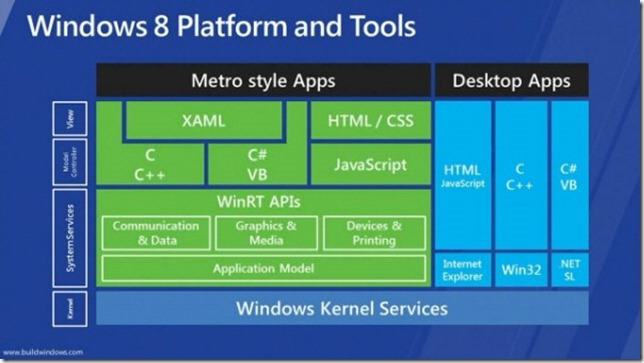
\includegraphics[scale=0.90]{images/win8-platform-and-tools_thumb.jpg}
\caption[WinRT Architektur: Grafik von Microsoft. Quelle: \cite{dse11}]{WinRT Architektur, Grafik von Microsoft}\label{Abb1}
\end{figure}
\newline
Einer der Hauptkritikpunkte war dabei, dass nicht klar herauszulesen war, in welcher Beziehung die .NET API zur WinRT API steht, und ob die langjährig verwendete .NET API nun komplett ersetzt wird. \cite{dse11}
\newline
\newline
Tatsächlich läuft die neue COM basierte Windows Runtime nur parallel zum API-Set von .NET. Man kann weiterhin in C\# programmieren und die Standard-APIs auch wie gewohnt aufrufen, im Hintergrund mapped der Compiler die Aufrufe allerdings und leitet sie an entsprechende WinRT Funktionen weiter.
\newline
\newline
Die WinRT APIs sind dabei in WinMD-Files definiert, die dasselbe Dateiformat (ECMA-335) besitzen, wie die .NET Framework Assemblies. Trotz dieses gemeinsamen Formates ähneln sich die Metadaten-Files nur und sind nicht ident, was unter anderem den Grund hat, dass die WinRT und .NET komplett unterschiedliche Datentypen besitzen, welche ebenfalls bei Bedarf aufeinander gemapped werden müssen.
\newline
\begin{figure}[htbp]
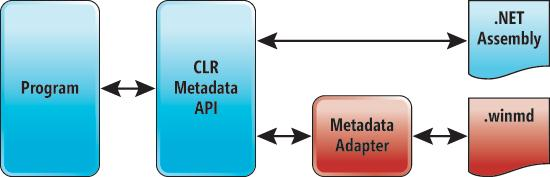
\includegraphics[scale=1]{images/farkas_winrt_clr.jpg}
\caption[The Metadata Adapter. Quelle: \cite{sfar12}]{Metadata Adapter}\label{Abb2}
\end{figure}
\newline
Damit das funktioniert, müssen Compiler auch WinMD Files lesen können, was standardmäßig natürlich nicht der Fall ist, da die Compiler im Normalfall vor der Entwicklung von WinRT eingesetzt wurden. Aus diesem Grund wurde der Metadata Adapter eingeführt, wie in \ref{Abb2} ersichtlich.
\newline
Die Common Language Runtime (CLR) Metadata API wird von verschiedenen Compilern, wie auch von Visual Studio verwendet, um .NET Metadata Files auszulesen.
Der Metadata Adapter hat nun die Aufgabe, die WinMD-Files für die CLR Metadata API zu übersetzen, damit diese gelesen werden können, als ob sie selbst .NET Assemblies wären.
\cite{sfar12}
\newline
\newline
Aus Gründen des beschränkten Umfangs dieser Arbeit wird der interessierte Leser an dieser Stelle jedoch auf die angegebenen Quellen verwiesen. Die APIs von WinRT finden an späterer Stelle in dieser Arbeit noch einmal detailliert Erwähnung.
 
\section[Neue Hardware und Tablets]{Neue Hardware und Tablets}
WinRT Applikationen laufen immer noch auf bisherigen Desktopcomputern und Laptops (solange auf diesen Windows 8 oder Windows RT installiert ist), erstmalig sind aber Anwendungen, die für ein Windows-Betriebssystem geschrieben wurden, auch auf Tablets ausführbar.
\newline
Diese Geräte werden gewöhnlich ohne Maus und Tastatur bedient, die Toucheingabe muss genügen. Um trotzdem eine ausreichende Bedienbarkeit zu gewährleisten, hat Microsoft Mindest-Hardwareanforderungen festgeschrieben, die ein Hersteller erfüllen muss, um ein Gerät mit einem der neuen Betriebssysteme auf den Markt bringen zu dürfen.
\newline
Diese sind in drei PDF-Dokumenten nachlesbar, die insgesamt 1258 Seiten umfassen. Um ein Beispiel zu nennen: User verwenden gewöhnlich die Tastenkombination Ctrl + Alt + Del am Startscreen, um sich anschließend anmelden zu können. Bei Geräten, die keine Tastatur mit sich führen, muss diese Funktionalität ebenfalls gewährleistet bleiben. Aus diesem Grund müssen solche Geräte eine Windowstaste und einen Power-Knopf besitzen, welche, in Kombination gedrückt, die selbe Funktion auslösen.
\newline
\newline
Die Windows-Taste spielt also vermehrt eine wichtige Rolle für Microsofts neue Usability-Strategie und ist neben dem Power-Knopf und den Lautstärkereglern auch die einzige physische Taste, die jedes Gerät implementiert haben muss. \cite{hw12}, S.89f
\newline
\newline
Näher wird in dieser Bachelorarbeit jedoch nicht auf die Hardwareanforderungen eingegangen, der interessierte Leser kann die detaillierten Informationen aber über die von Microsoft zur Verfügung gestellten PDFs abfragen.
% http://msdn.microsoft.com/library/windows/hardware/hh748188

%-------------------------------------------------------------------------------------------------------------------------------------------------------

\chapter[Layout]{Layout}
Im Rahmen dieser Bachelorarbeit wird eine einfache Line of Business Applikation namens \textit{Practitioner Mobile} erstellt. Auf diese wird vereinzeilt bereits in diesem Kapitel zu praktischen Demonstrationszwecken eingegangen. Der genaue Zweck dieser Applikation wird in einem späteren Kapitel erläutert, in diesem stehen hingegen Basics im Bereich des Layouts einer typischen Windows 8 / Windows RT Applikation im Vordergrund.
\section[XAML]{XAML}\label{sec:XAML}
Die Extensible Application Markup Language (XAML) ist kein neues Konzept, das für WinRT entwickelt wurde. Vielmehr existiert diese bereits seit .NET 3.0 und wurde erstmalig für die Benutzeroberflächenerstellung bei Windows Presentation Foundation (WPF) Anwendungen eingesetzt. Grund für die Einführung war der Wunsch einer besseren Trennung von User Interface (UI) Design und Logik, wobei die Oberfläche prinzipiell immer noch rein programmatisch erstellt werden kann.
\newline
\newline
XAML basiert, wie der Name bereits suggeriert, auf der Extensible Markup Language (XML), wobei den Elementen Klassen im Code zugeordnet werden. Attribute werden als Properties und Events interpretiert. Um verschiedene Klassen dabei unterscheiden und kategorisieren zu können, werden diese in Namespaces eingeteilt, die im XAML Code deklariert werden müssen. 
\cite{wpf10}, S.141ff
\newline
\newline
Zwei Namespaces sind dabei besonders hervorhebenswert: 
\begin{itemize}
\item \textit{http://schemas.microsoft.com/winfx/2006/xaml/presentation}:
\newline
In diesem Namespace finden sich die meisten der Standard UI Elemente. Elemente in diesem Namespace müssen als einzige beim Einfügen in XAML Code kein Kürzel angeben, um sich von anderen Namespaces zu unterscheiden.
\newline
\newline
Beispiele: Grid, Button, TextBlock.
\item \textit{http://schemas.microsoft.com/winfx/2006/xaml}:
\newline
Das ist der Namespace für XAML spezifische Elemente, in welchem spezielle XAML-Parser Direktiven definiert werden.
\newline
Diesen wird üblicherweise ein x vorgestellt.
\newline
Klassische Controls, wie man sie unter einem UI Namespace eigentlich erwarten würde, findet man hier nicht.
\newline
\newline
Beispiele: Class, Name, Key.
\end{itemize} 
Natürlich können neben den Standard Controls auch eigene je nach Bedarf ergänzt werden. Diese sind dann in einem eigenen zu definierenden Namespace zu finden. \cite{ana12}, S.29f
\newline
\newline
Ein aus Visual Studio frisch erzeugtes Windows 8 / Windows RT Projekt in XAML Code sieht folgendermaßen aus:
\begin{lstlisting}[caption={XAML einer neu erzeugten Windows 8 Applikation }\label{lst:1},captionpos=t]
<Page
    x:Class="PractitionerMobile.MainPage"
    xmlns="http://schemas.microsoft.com/winfx/2006/xaml/presentation"
    xmlns:x="http://schemas.microsoft.com/winfx/2006/xaml"
    xmlns:local="using:CustomNamespace"
    xmlns:d="http://schemas.microsoft.com/expression/blend/2008"
    xmlns:mc="http://schemas.openxmlformats.org/markup-compatibility/2006"
    mc:Ignorable="d">

    <Grid Background="{StaticResource ApplicationPageBackgroundThemeBrush}">

    </Grid>
</Page>

\end{lstlisting}
Die beiden zuvor erwähnten Namespaces sind an dieser Stelle wiederzufinden.
\newline
Wie man anhand des \textit{local} Namespaces sieht, können eigene Namespaces ganz simpel durch das Voranstellen einer \textit{using} Direktive hinzugefügt werden. Dieser eigene Namespace muss natürlich auch im Code Behind vorhanden sein.
\newline
\textit{CustomNamespace} ist dabei der Namespace der Klasse oder Klassen, in welchen eigene Funktionen definiert sind. Die Rolle des \textit{Grid} Elements wird später in dieser Arbeit erklärt.
\newline
\newline
Näher wird an dieser Stelle aus Platzgründen nicht auf die Grundlagen von XAML eingegangen, diese werden zum weiteren Verständnis dieser Bachelorarbeit vorrausgesetzt und können bei Bedarf in den erwähnten Quellen selbst erarbeitet werden.

\section{Struktur einer Applikation}
Jedes XAML File besitzt auch ein Code Behind File, in welchem der Großteil der Logik ausprogrammiert wird. So wird die in \ref{sec:XAML} erwähnte Trennung dieser vom UI Design realisiert.
\newline
\newline
In den Files App.xaml und dessen Code Behind File App.cs können Elemente definiert werden, die seitenunabhängig zur Verfügung stehen sollen. In letzterem sind auch globale Events wie das Starten oder das Beenden einer Applikation abfangbar.
\newline
\newline
Bilder finden sich im Folder \textit{Assets}, Styles im Folder \textit{Common} wieder.
\newline
\begin{figure}[htbp]
\centering
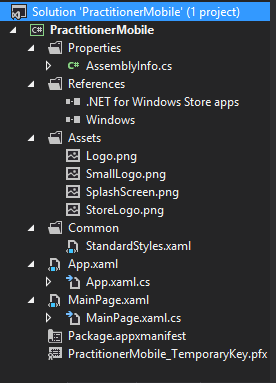
\includegraphics[scale=1]{images/filetree.png}
\caption[File Tree eines neu erzeugten Windows 8 / Windows RT Projekts]{File Tree}\label{Abb3}
\end{figure}
\newline
Der klassische Aufbau eines frisch generierten Solution ist in Abbildung \ref{Abb3} ersichtlich.
\newpage
Wählt man beim Erstellen des Projekts kein leeres Projekt aus, sondern eines der anderen verfügbaren Templates, wird etwas mehr (XAML) Code automatisch generiert. Wählen kann man zwischen einer Grid App oder einer Split App, die bereits Listen von Elementen beinhalten und auch die Navigation zu einer Detailseite ist bereits vorimplementiert. In der Practitioner Mobile Applikation wird von diesen Templates jedoch kein Gebrauch gemacht, alle Elemente können auch später bei Bedarf ergänzt werden.

\section[Portrait und Landscape]{Portrait, Landscape und Snapped View}
Die Tatsache, dass sich bei Tablets nicht nur die Bildschirmgröße, sondern auch die Orientierung ändern kann, stellt Entwickler vor eine zusätzliche Herausforderung. Außerdem hat Microsoft in seinen neuen Betriebssystemen den Snapped View integriert, welcher es ermöglicht, zwei Anwendungen gleichzeitig am Bildschirm anzuzeigen, normalerweise nimmt eine Anwendung immer den gesamten Bildschirm ein. Dieser Snapped View eröffnet viele neue Möglichkeiten, man kann in etwa einen Texteditor und ein Wörterbuch parallel laufen lassen, um beim Schreiben eines fremdsprachlichen Textes ein Wort schnell und einfach nachschlagen zu können. 
\newline
Abbildung \ref{Abb4} visualisiert dieses Beispiel anhand zweier bereits im Windows Store verfügbaren Apps: Microsofts OneNote Notizbuch, und dem Übersetzungstool Leo. In den Snapped View kann nur im Landscape Mode gewechselt werden und ist verpflichtend für jede Applikation.
\newline
\newline
Um Entwicklern die Arbeit zu erleichtern, bestimmt Microsoft eine Mindestbreite für die verschiedenen Viewstates. Für die beiden Fullscreen Views (Portrait und Landscape) wird so eine Mindestauflösung von 1024x768 Pixel garantiert. Um den Snapped View zu unterstützen, muss das Gerät bereits eine Breite von 1366 Pixel aufweisen - 320 Pixel extra für die gesnappte App und 22 Pixel für den Splitter zwischen den beiden Applikationen. \cite{ana12}, S.65ff
\begin{figure}[htbp]
\centering
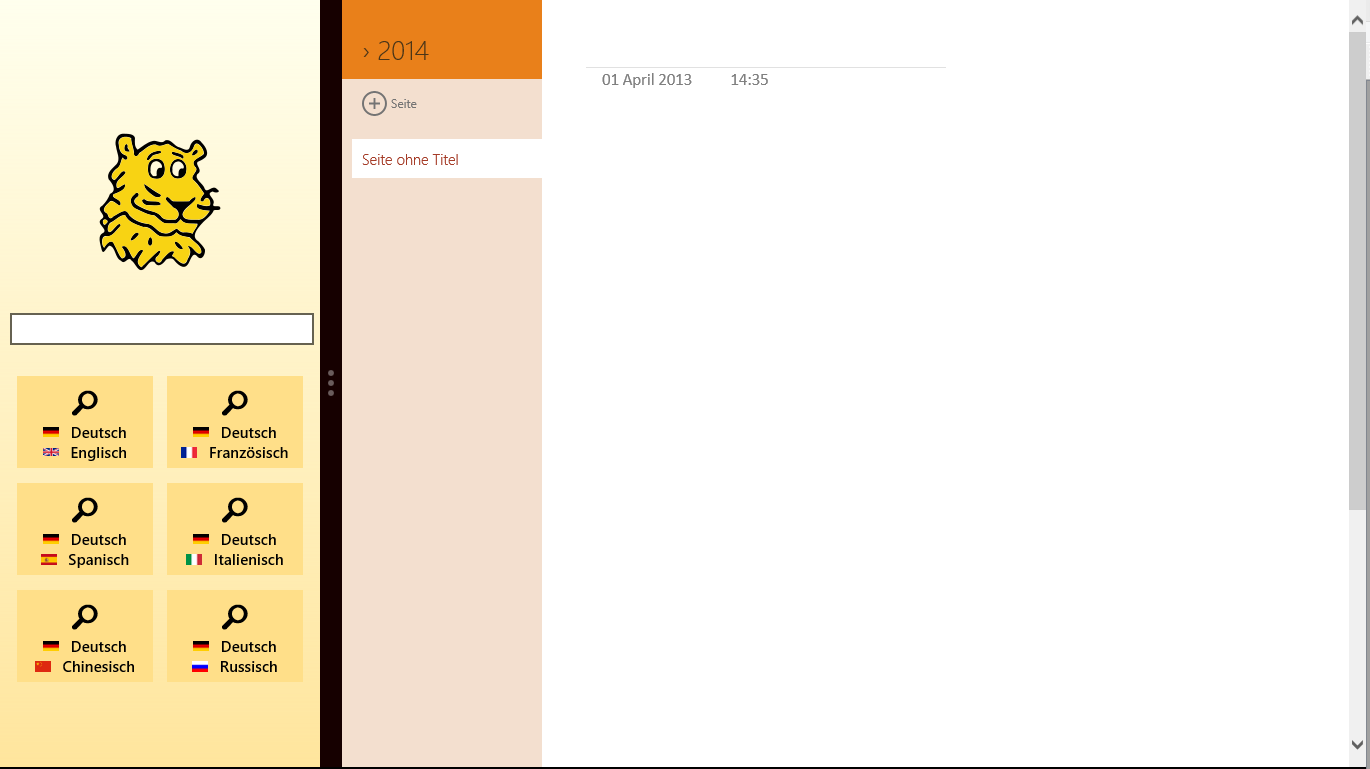
\includegraphics[scale=0.4]{images/snapped.png}
\caption[Snapped View]{Snapped View}\label{Abb4}
\end{figure}

\section[Splash Screen]{Splashscreen}
Beim Öffnen der Applikation wird ein Startbildschirm, der so genannte Splash Screen, angezeigt. Dieser ist statisch und kann durch ein eigenes Bild ersetzt werden, in dem man das File \textit{SplashScreen.png}, ersichtlich in Abbildung \ref{Abb3}, durch die gewünschte Grafik ersetzt.
\newline
Die Zeit, in welcher der Splashscreen gezeigt wird, kann der Entwickler dazu nutzen, um Vorbereitungsarbeiten für seine Applikation zu treffen. Diese dürfen die Zeitspanne von fünf Sekunden nicht überschreiten.
\cite{ana12}, S.10f

\section[Controls]{Controls}\label{ref:controls}
Wie jedes XML basierte Dokument besitzt auch ein XAML File ein Root-Element, bei einer WinRT Seite ist dies \textit{<Page>}. Innerhalb dieses Elements finden sich dann verschachtelt, wie in einem XML Dokument, verschiedenste weitere Elemente.
\newline
\subsection[Panels]{Panels}\label{ref:panels}
Ein Panel ist ein Wrapper-Element - ein so genanntes Content Control -, das für das Basis-Layout seiner Kindelemente verantwortlich ist.
\newline
Die am häufigsten verwendetsten Panels sind:
\begin{itemize}
\item \textit{Canvas}:
\newline
Einfaches, dafür performantes Panel.
\item \textit{StackPanel}:
\newline
Optimal, um Elemente horizontal oder vertikal aneinanderzufügen.
\item \textit{Grid}:
Eines der am häufigsten verwendeten und mächtigsten Panels, mit einer Tabelle vergleichbar.
\newline
Elemente können in zuvor definierte Zeilen und Spalten eingefügt und somit präzise positioniert werden.
\end{itemize}
\cite{ana12}, S.71ff

\subsection[Aufzählungen]{Aufzählungen}
Im Gegensatz zu den eben in \ref{ref:panels} vorgestellten Panels, besitzen so genannte Items Controls, zu denen Aufzählungscontrols gehören, zusätzliche Properties: \textit{SelectedIndex}, \textit{SelectedItem} und \textit{SelectedValue}. Diese machen es möglich, in Aufzählungen bestimmte Elemente auszuwählen, und somit in weiterer Folge nach Elementen zu suchen, zu aktualiseren, zu löschen oder neue Elemente hinzuzufügen.
\newline
Diese Properties werden dabei automatisch synchronisiert, der Programmierer muss sich also in etwa nicht darum kümmern, den Index beim Ändern einer Aufzählung zu verändern.
\newline
\newline
Als übergeordnetes Element besitzen Items Controls ebenfalls Panels, die meisten dieser besitzen aber zusätzlich eine Art von Virtualisierung, um Performanceoptimierungen zu erreichen. Besonders bei einer großen Anzahl von Elementen in diesen Listen ist eine deutliche Effizienzsteigerung bemerkbar.
\newline
\newline
Die bekanntesten Aufzählungscontrols sind:
\begin{itemize}
\item \textit{ComboBox}: Die ComboBox ist ein Control, die es erlaubt, aus mehreren verfügbaren Elementen genau eines aus einer Drop Down Liste auszuwählen. Sie nimmt dabei nicht viel Platz am UI weg, da sie im geschlossenen Zustand nur das aktuell gewählte Element anzeigt und wird aus diesem Grund gerne verwendet. Neue Elemente zu einer bestehenden ComboBox kann der User allerdings vom UI aus nicht.
\newline
\item \textit{ListBox}: Die ListBox ähnelt der CoboBox, mit dem Unterschied, dass alle Elemente am UI angezeigt werden, und dass man - je nach Konfiugration - auch mehrere Elemente auf einmal auswählen kann.
\newline
\item \textit{ListView}: Die ListView ist der ListBox sehr ähnlich und stellt sozusagen eine für Touch optimierte Variante derselben dar.
\newline
\item \textit{GridView}: Das GridView hat wiederum viele Gemeinsamkeiten mit der ListView. Unterschiede findet man nur in der Darstellung der Elemente: während die ListView standardmäßig vertikal scrollt, orientiert sich die GridView sich an der Horizontalen. Außerdem wird jeden Element so viel Platz gegeben, wie dem größten Element in der Aufzählung. Alle anderen Elemente passen ihre Darstellung also diesem an.
\end{itemize}
 \cite{ana12}, S. 207ff

\subsection[TextBlock]{TextBlock}
Das TextBlock wird dazu verwendet, um Text im UI anzuzeigen. Dabei stehen dem Control viele verschiedene Formatierungsmöglichkeiten als Properties zur Verfügung. Verändern kann man so unter anderem die Schriftart, die Schriftgröße, die Farbe des Textes oder dessen Formatierung.
\newline
Dabei muss innerhalb eines TextBlocks nicht der ganze Textstring gleich formatiert werden. Man kann diesen durchaus in einzelne Bereiche, so genannte \textit{Run}-Blöcke aufteilen und getrennt voneinander bearbeiten:
\newline
\begin{lstlisting}[caption={Run-Blöcke in einem TextBlock}\label{lst:RunTextBlock},captionpos=t]
<TextBlock>
	<Run FontSize="10">Dieser Text</Run>
	<Run FontSize="20">kann seperat</Run>
	<Run FontSize="30">formatiert werden.</Run>
</TextBlock>
\end{lstlisting}
Setzt man das Property \textit{IsTextSelectionEnabled} auf \textit{true}, kann der User Text in TextBlocks auswählen und anschließend zum Beispiel in die Zwischenablage kopieren.
\cite{ana12}, S. 227ff

\subsection[TextBox]{TextBox}
Das TextBox Control wird an den Stellen im UI verwendet, in denen der User Text eingeben können soll. Bekommt dieses Control den Fokus, öffnet sich die Software-Tastatur automatisch (sofern es sich um ein Touch-fähiges Gerät handelt). Rechtschreibprüfung unterstützt das Control von Haus aus, genauso wie das Anbieten von Vorschlägen für die Eingabe. \cite{ana12}, S. 240ff

\section[Semantic Zoom]{Semantic Zoom}
Semantic Zoom wird die Möglichkeit genannt, aus einer großen Anzahl von Elementen - wie etwa in Aufzählungen - hinauszuzoomen, um einen besseren Überblick über die verfügbaren Elemente zu bekommen, diese zu gruppieren, oder ähnliches. Windows verwendet diese Funktionalität bereits am Startbildschirm, auf welchem alle verfügbaren Apps angezeigt werden.
\newline
\newline
Wie bei den meisten Möglichkeiten, die WinRT Applikationen beherrschen, macht diese Option nicht überall Sinn. Gerade aber wenn es darum geht, sich in einer Vielzahl von Elementen zurecht zu finden, kann diese aber sehr hilfreich sein. \cite{ana12}, S.223ff

\section[Entwicklung von eigenen Controls]{Entwicklung von eigenen Controls}
Wie auch schon bei WPF, stehen mit XAML dem Entwickler eine große Anzahl von Möglichkeiten für das Erstellen von eigenen Controls zur Verfügung.
\subsection[Dependency Properties]{Dependency Properties}\label{ref:dependencyprops}
Dependency Properties zählen zu den wichtigsten Elementen in XAML. Von einem normalen Property unterscheiden sie sich dabei nur durch XAML-spezifische Zusatzfunktionalitäten: Änderungsnotifikationen an gebundene Elemente, Wertevererbung an Kindelemente und die Unterstützung für mehrere Provider. 
Man erklärt die Motivation für Dependency Properties und die Funktion der automatischen Änderungsnotifikation am Besten an einem einfachen Beispiel.
\newline
\newline
Dafür wird eine Art Basis-Button Control gebaut, welches - wie der Standard-Control Button - erkennen soll, ob er sich gerade in gedrücktem oder ungedrücktem Zustand befindet. Es wird eine neue Klasse namens \textit{BaseButton} erstellt, die wie Button auch von \textit{ContentControl} ableitet, um möglichst viele Gemeinsamkeiten zu behalten. Unser Button soll ein neues Property namens \textit{IsPressed} bekommen, anhand dem er erkennen kann, ob er aktiviert oder deaktivert wurde. Ein Klick auf ihn soll dabei seinen Zustand ändern.
\newline
\newline
\begin{figure}[htbp]
\centering
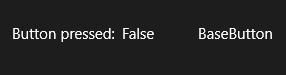
\includegraphics[scale=1]{images/buttonpressed_false.png}
\caption[Button nicht gedrückt]{Button nicht gedrückt}\label{Abb5}
\end{figure}
\newline
\newline
\begin{figure}[htbp]
\centering
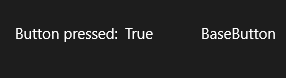
\includegraphics[scale=1]{images/buttonpressed_true.png}
\caption[Button gedrückt]{Button gedrückt}\label{Abb6}
\end{figure}
\newline
Der entsprechende XAML Code, gekürzt auf die wichtigsten Elemente, sieht folgendermaßen aus:
\newline
\begin{lstlisting}[caption={XAML eines neu erstellten Controls }\label{lst:2},captionpos=t]
<Page
[...]
xmlns:pc="using:PractitionerMobile.Controls">
[...]
<TextBlock Text="Button pressed:" />
<TextBlock Text="{Binding ElementName=baseButton, Path=IsPressed}" />
<pc:ButtonBase Name="baseButton" Content="BaseButton" 
	Tapped="baseButton_Tapped" />
[...]
</Page>
\end{lstlisting}
Wie in Listing \ref{lst:2} zu erkennen ist, wird unsere Klasse \textit{ButtonBase} nicht einfach so eingefügt, sondern bekommt einen Namespace vorangestellt. Dieser muss im XAML File innerhalb des Page-Elements ebenfalls deklariert werden.
\newline
\newline
Der Text des zweiten TextBlock Elements bindet sich an unseren gerade erstellten Button und zeigt den Wert dessen IsPressed Value an, welcher sich bei jedem Klick auf \textit{BaseButton} ändert. Die Grundlagen des XAML Databindings sind nicht Gegenstand dieser Arbeit, vielmehr sollen die Möglichkeiten aufgezeigt werden, die Entwicklern mit XAML und C\# zur Verfügung stehen.
\newline
\newline
Schlussendlich muss noch der Code Behind implementiert werden, welcher so aussieht, wie in Listing \ref{lst:3} dargestellt.
\begin{lstlisting}[caption={Für Dependency Properties benötigter Code}\label{lst:3},captionpos=t]
MainPage.xaml.cs:

using CustomBaseButton = PractitionerMobile.Controls.ButtonBase;
[...]
private void baseButton_Tapped(object sender, TappedRoutedEventArgs e)
{
        CustomBaseButton button = (sender as CustomBaseButton);

        if(button.IsPressed)
        {
            button.SetValue(CustomBaseButton.IsPressedProperty, false);
        }
        else
        {
            button.SetValue(CustomBaseButton.IsPressedProperty, true);
        }
 }
[...]


ButtonBase.cs:

[...]
public class ButtonBase : ContentControl
{
    public bool IsPressed
    {
        get { return (bool)GetValue(IsPressedProperty); }
        set { SetValue(IsPressedProperty, value); }
    }

    public static readonly DependencyProperty IsPressedProperty = 
        DependencyProperty.Register("IsPressed", typeof(bool),
		 typeof(ButtonBase), new PropertyMetadata(false, 
			OnIsPressedChanged));

    private static void OnIsPressedChanged(DependencyObject d, 
					DependencyPropertyChangedEventArgs e)
    {
        Debug.WriteLine("button pressed: " + e.NewValue);
    }
}
[...]
\end{lstlisting}
Im File \textit{MainPage.xaml.cs} wird mittels der SetValue-Methode der Wert des in \textit{ButtonBase.cs} definierten Dependency Properties umgesetzt.
\newline
Der .NET Property Wrapper \textit{public bool IsPressed} ist dabei rein optional, ebenso wie der Property Changed-Callback \textit{OnIsPressedChanged}, in dem man zusätzliche Logik verpacken könnte. \cite{ana12}, S. 102f

\subsection[Attached Properties]{AttachedProperties}
Attached Properties unterscheiden sich von Dependency Properties in der Funktionsweise und Implementierung nur gering, und zwar hauptsächlich dadurch, dass diese \begin{quote}[...] nicht auf Objekten der Klasse gesetzt [werden], die das \textit{DependencyProperty}-Feld und damit den \textit{Schlüssel} zum eigentlichen Wert besitzt, sondern auf Objekten anderer Klassen.\end{quote}
Somit kann man in etwa von einem Button-Control aus, das ein TextBox-Control beinhaltet, direkt auf dieses zugreifen und dessen Wert verändern. Näher wird auf Attached Properties aufgrund der großen Ähnlichkeit zu Dependency Properties nicht eingegangen. \cite{wpf10}, S.413

\subsection[Property Wertevererbung und mehrere Provider]{Property Wertevererbung und mehrere Provider}
Wird auf einem Parent-Element ein Property, zum Beispiel die Schriftgröße eines Textes, auf einen bestimmten Wert gesetzt, kann es die Eigenschaft auch auf seine Kindelemente übertragen. Ob das geschieht oder nicht, hängt jedoch von einigen 
Faktoren ab. Setzt das Kindelement seinerseits einen Wert für dasselbe Property, wird der Wert des Parents überschrieben. 
\newline
\newline
Auch sonst gibt es eine definierte Prioritätsliste, welche genau angibt, welcher Wert für ein Property nun tatsächlich verwendet werden soll. Wenn in etwa gerade eine Animation durchgeführt wird, hat der in dieser gesetzte Wert immer Vorrang. Die genaue Prioritenliste sieht wie folgt aus:
\begin{enumerate}
\item Aktive Animationen
\item Lokale Werte
\item Template Properties
\item Style-Setters
\item Property Wertevererbung
\item Default-Wert
\end{enumerate}
Über Styles und Templates wird an späterer Stelle dieser Arbeit noch geschrieben.
\cite{ana12}, S. 104ff

\subsection[Styles]{Styles}\label{ref:styles}
Angenommen, man will das Aussehen eines Buttons verändern. In diesem Fall setzt man im XAML-File die entsprechenden Properties und bekommt so einen Button, der genauso gerendert wird, wie man es möchte.
\newline
Wenn man nun aber nicht nur eines Controls ändern möchte, sondern eine ganze Reihe von einem bestimmten Control, wird es mühsam und unübersichtlich: man müsste bei jedem einzelnen die selben Properties setzen, was das XAML-File unnötig aufbläht.
\newline
An dieser Stelle kommen Styles ins Spiel.
\newline
\newline
Styles machen es möglich, mehrere Eigenschaften auf einmal zu gruppieren und auf alle Elemente eines Typs einfach anzuwenden. Definiert werden Styles direkt auf Controls, sodass alle in der Hierarchie darunterliegenden Kindelemente dieses Typs besagte Eigenschaften nutzen können. \cite{ana12}, S. 410ff
\newline
\newline
In Listing \ref{lst:styles} ist dargestellt, wie ein Style für TextBlock-Elemente innerhalb der definierten ListView definiert wird, der die \textit{FontWeight} auf \textit{Bold}, die \textit{Foreground}-Farbe auf \textit{Red}, und ein \textit{Padding} von links auf 20 setzt.
\newline
Der Style wird dazu als Resource der ListView definiert und in den gewünschten TextBlock-Elementen mit \textit{Style="\{StaticResource ListViewTextBlockStyle\}"} angewendet.
\newline
\begin{lstlisting}[caption={Definition eines Styles}\label{lst:styles},captionpos=t]
<ListView Name="elementPanel">
   <ListView.Resources>
       <Style x:Key="ListViewTextBlockStyle" TargetType="TextBlock" >
           <Setter Property="FontWeight" Value="Bold" />
           <Setter Property="Padding" Value="20,0,0,0" />
           <Setter Property="Foreground" Value="Red" />                         
        </Style>
   </ListView.Resources>
   <ListViewItem>
       <TextBlock Text="TextBlock 1"
	 Style="{StaticResource ListViewTextBlockStyle}" />
   </ListViewItem>
   <ListViewItem>
       <TextBlock Text="TextBlock 2" />
   </ListViewItem>
</ListView>
\end{lstlisting}
Nur das erste TextBlock-Control bekommt den Style zugewiesen, der zweite behält somit seine Default-Formatierung, wie in Abbildung \ref{img:styles} gezeigt wird.
\begin{figure}[htbp]
\centering
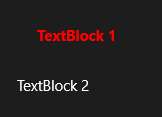
\includegraphics[scale=1]{images/styles.png}
\caption[Styles]{Styles}\label{img:styles}
\end{figure}
Lässt man \textit{x:Key} und \textit{x:Name} weg, verzichtet also darauf, dem Style einen Identifier zu geben, wird der Style auf alle Elemente des definierten Typs angewendet.
\newline
\newline
Ein Control kann einen durch Styles gesetzten Property-Wert auch überschreiben, indem es einfach einen anderen Wert für diesen setzt.
\newline
\newline
Schon beim Anlegen einer neuer WinRT-Solution wird das File \textit{Common/StandardStyles.xaml} erstellt. In diesem File finden sich einige Styles bereits vordefiniert, die nur noch im XAML eingebunden werden müssen. Styles können dabei auch voneinander erben, was wieder einiges an Schreibarbeit erspart und den Code übersichtlicher macht.
\newline
\newline
WinRT-Applikationen können unter drei verschiedenen Themes laufen: \textit{Default} (entspricht schwarz), \textit{Light} (entspricht weiß) und \textit{High Contrast} (entspricht weißem Text auf schwarzem Hintergrund).
\newline
Schlussendlich ist es auch möglich, für jedes dieser Themes einen anderen Style zu definieren. \cite{ana12}, S. 413ff

\subsection[Templates]{Templates}
Die Einführung von XAML hat es ermöglicht, die Darstellung eines Objekts im UI vollständig von dessen Logik zu trennen. Somit kann in etwa die Darstellung eines Buttons nach Belieben verändert werden, ohne dass sich an der Funktionalität etwas ändert.
\newline
Das vorherige Unterkapitel \ref{ref:styles} hat gezeigt, wie einfach es ist, mittels Styles das Erscheinungsbilds eines Controls zu verändern. Dies hat sich aber auf einfache Properties beschränkt, will man das Design von Grund auf neu schreiben, bedient man sich am besten Templates.
\newline
\newline
Es gibt mehrere verschiedene Arten von Templates, drei davon erben von der Klasse \textit{FrameworkTemplate}: \textit{ControlTemplate}, \textit{DataTemplate} und \textit{ItemsPanelTemplate}.

\subsubsection[ControlTemplate]{ControlTemplate}\label{ref:controltemplate}
ControlTemplates ermöglichen es, das Aussehen eines Controls vollkommen nach Belieben neu zu gestalten. Ein Button muss somit nicht mehr rechteckig sein, sondern kann durchaus auch als Kreis oder Ellipse dargestellt werden. Die Funktionalität bleibt dabei erhalten, er verfügt zum Beispiel immer noch über sein \textit{OnClick}-Event.
\newline
\newline
ControlTemplates kann man direkt im XAML definieren, aber auch wie Styles in ein Resources-File auslagern. Ebenfalls möglich ist es, in der Definition eines Styles (zum Beispiel im File \textit{StandardStyles.xaml})  ein Template zu inkludieren.
\newline
\newline
Ein Problem taucht aber dennoch auf: wenn man das Design eines Controls, zum Beispiel eines Buttons, neu schreibt, woher weiß dieser, an welcher Stelle er sein Content-Property anzeigen soll? Angenommen, er würde als Content den String \textit{Mein Button} und als Design einen Kreis statt ein Rechteck gesetzt haben - der String würde nie angezeigt werden.
\newline
Um dieses Problem zu lösen, muss man in die Template-Definition des Buttons ein Control definieren, welches diese Aufgabe übernimmt. Das könnte eine TextBox sein, generischer ist allerdings eine ViewBox - der Content beschränkt sich dann nicht nur auf Text, sondern könnte ebensogut ein Bild oder ein sonstiges Element sein. Das Template könnte dann so aussehen, wie in Listing \ref{lst:templates}.
\begin{lstlisting}[caption={Definition eines Templates. Modifiziert von \cite{ana12}, S.421}\label{lst:templates},captionpos=t]
<Button Content="Mein Button">
   <Button.Template>
      <ControlTemplate TargetType="Button">
	[...]
	<ViewBox Width="100" Height="100">
	   <ContentControl Margin="20"
		Content="{TemplateBinding Content}" />
	</ViewBox>
	[...]
      </ControlTemplate>
   </Button.Template>
</Button>
\end{lstlisting}
Durch das explizite Setzen des Contents auf ein Control kann das Problem also gelöst werden. XAML bedient sich hierbei an einem Konzept, das als \textit{DataBinding} bekannt ist und bereits im Abschnitt \ref{ref:dependencyprops} verwendet wurde. Die Funktionsweise dieses Konzepts wird in dieser Bachelorarbeit nicht detailliert erläutert.
\cite{ana12}, S. 418ff

\subsubsection[Visual States]{Visual States}\label{ref:visualstates}
Bisher wurde erklärt, wie das Aussehen eines Controls verändert werden kann. Ein solches kann aber auch unterschiedliche Zustände besitzen, bei einem Button würde so in etwa zwischen gedrückt und nicht gedrückt unterschieden werden. Wenn dieser je nach Zustand eine andere Darstellung besitzen soll, kommen Visual States ins Spiel.
\newline
\newline
Zustände, die ein Control annehmen kann, werden in so genannte \textit{State Groups} gruppiert, die einander ausschließen. Definieren kann man solche hierarchisch direkt unter dem gewünschten Control-Root-Element mit dem Attached Property \textit{VisualStateManager.VisualStateGroups}, welche wiederum \textit{VisualStateGroup}-Elemente und abermals eine hierarchische Ebene darunter \textit{VisualStates} enthalten.
\newline
Das \textit{x:Name} Attribut einer VisualStateGroup entspricht dabei einer möglichen Zustandsgruppe (zum Beispiel \textit{CommonStates}), das eines VisualStates einem möglichen Zustand (zum Beispiel \textit{Focused}). Welche Zustände es gibt, ist individuell pro Control verschieden und als Attribut auf der Klasse im Code Behind definiert.
\newline
\newline
Übergänge zwischen verschiedenen Visual States werden gerne durch Animationen durchgeführt, für die man das \textit{Storyboard}-Element verwendet. \textit{Visual Transitions} erleichtern dabei viele Animationsvorgänge, indem man nur angeben muss, welches Property sich von welchem auf welchen Wert ändern soll. Die Animation wird dann berechnet und automatisch durchgeführt. Auch gewünschte Verzögerungen können dabei angegeben und somit die Schnelligkeit der Transformation kontrolliert werden.
\newline
Auf Animationen wird in dieser Bachelorarbeit aus Platzmangel jedoch nicht näher eingegangen. \cite{ana12}, S.428ff

\subsubsection[DataTemplate]{DataTemplate}\label{ref:datatemplate}
Oftmals steht im Vorhinein noch nicht fest, welche Elemente eine Aufzählung tatsächlich beinhalten wird, da diese erst später programmatisch und durch Data Binding hinzugefügt werden. Wenn es die Elemente aber im XAML noch nicht gibt, kann man sie auch nicht stylen oder Properties setzen.
\newline
\newline
Um mehrere Objekte innerhalb einer Aufzählung gleichzeitig zu formatieren, werden aus diesem Grund Data Templates eingesetzt. Diese werden hierarchisch direkt unter dem gewünschten Aufzählungscontrol definiert. \cite{ana12}, S.447
\newline
\newline
Für eine ListView würde ein DataTemplate in etwa so aussehen, wie in Listing \ref{lst:datatemplate} dargestellt.
\begin{lstlisting}[caption={Data Template}\label{lst:datatemplate},captionpos=t]
<ListView ItemsSource="{Binding Patients}>
   <ListView.Resources>
      <Style x:Key="ListViewTextBlockStyle" TargetType="TextBlock" >
         <Setter Property="FontWeight" Value="Bold" />
         <Setter Property="Padding" Value="20,0,0,0" />                         
      </Style>
   </ListView.Resources>

   <ListView.ItemTemplate>
      <DataTemplate>
          <TextBlock Text="{Binding Path=Name}"
		Style="{StaticResource ListViewTextBlockStyle}" />
      </DataTemplate>
   </ListView.ItemTemplate>
</ListView>
\end{lstlisting}
Die ListView bekommt hier ein \textit{DataTemplate} gesetzt, in dem für \textit{TextBlock}-Elemente ein neuer Style gesetzt wird. Dieser ist in diesem Codebeispiel nicht direkt gesetzt, sondern als Style innerhalb der ListView referenziert. Styles wurden im Unterkapitel \ref{ref:styles} erklärt. Der Content des TextBlock-Elements ist das \textit{Name}-Property eines Elements, das sich in eine Liste namens \textit{Patients} im CodeBehind befindet.

\subsubsection[ItemsPanelTemplate]{ItemsPanelTemplate}\label{itemspaneltemplate}
Mit einem ItemsPanelTemplate können Items innerhalb eines Controls einfach gestaltet werden. Im Gegensatz zum im Unterkapitel \ref{ref:datatemplate} vorgestellten Data Template, das sich auf Daten innerhalb einer Liste bezieht, werden hier nicht deren Properties verändert, sondern die des Listenelements selbst. Will man in etwa erreichen, dass sich jedes Listenelement innerhalb eines VirtualizingStackPanels befindet, das eine horizontale Orientierung hat, so kann man dies einfach durch in Listing \ref{lst:itemspaneltemplate} dargestelltes XAML erreichen.
\begin{lstlisting}[caption={ItemsPanelTemplate, aus \cite{ana12}, S.210}\label{lst:itemspaneltemplate},captionpos=t]
<ListBox>
   <ListBox.ItemsPanel>
      <ItemsPanelTemplate>
         <VirtualizingStackPanel Orientation="Horizontal" />
      </ItemsPanelTemplate>
   </ListBox.ItemsPanel>
</ListBox>
\end{lstlisting}
\cite{ana12}, S.210f

\section[Frameworks]{Frameworks}
Durch die Möglichkeit, nach Belieben mit XAML Custom Controls zu entwickeln, gibt es bereits erste Frameworks, die Sammlungen an individuellen Steuerelementen anbieten. Diese müssen nur noch aus der Visual Studio Toolbox in die eigene Solution mit Drag and Drop hineingezogen werden, und sind sofort so verwendbar, wie jedes andere Control auch.
\newline
\newline
Den Entwicklungsaufwand lassen sich die Hersteller der Custom-Lösungen natürlich auch etwas kosten, vor allem jetzt, wo WinRT-Applikationen noch am Anfang sind und noch nicht viel Konkurrenz am Markt ist.
\newline
Die Firma \textit{Syncfusion} bietet ein Set an Business-Controls zum derzeitigen Zeitpunkt um 199 Dollar an (\cite{syncfn}), deutlich teuerer kommen die Lösungen schon beim Konkurrenten \textit{Componenent One}: hier bezahlt man schon ab 895 Dollar für zusätzliche Elemente. Will man exklusiven Support dazu, wird es noch einmal teurer. \cite{cone}
\newline
\newline
Doch auch Gratis-Lösungen sind mittlerweile zu finden, wie in etwa das WinRT XAML Toolkit \cite{cptk}. Als Entwickler stehen einem also bereits einige Möglichkeiten zur Verfügung, wenn man ein Custom Control benötigt, aber keine Zeit und Energie für eine Eigenentwicklung investieren möchte.
\newline
\newline
Die im Rahmen dieser Bachelorarbeit erstellte Applikation Practitioner Mobile verwendet einen Kalender aus dem Control-Set von der Demoversion des \textit{Essential Studio for WinRT /XAML/} von Syncfusion. Das Control ist in Abbildung \ref{img:calendar} dargestellt.
\begin{figure}[htbp]
\centering
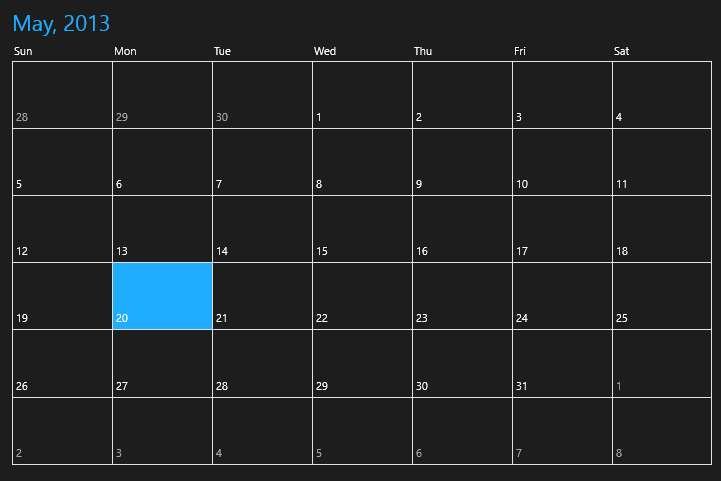
\includegraphics[scale=0.7]{images/calendar.png}
\caption[Syncfusion Kalender Control]{Syncfusion Kalender Control}\label{img:calendar}
\end{figure}

\section[Custom Control für Practitioner Mobile]{Custom Control für Practitioner Mobile}
Für die Anwendung Practitioner Mobile wurde ein eigenes Control entwickelt, das es erlaubt, für einen bestimmten Patienten einen Ordinationseintrag hinzuzufügen. Das Control ist in Abbildung \ref{img:customcontrol} ersichtlich. Der vollständige Code dazu befindet sich im Anhang unter \ref{app:customcontrol}.
\newline
\newline
 Die folgenden Schritte beziehen sich alle auf ein englische Version der Entwicklungsumgebung Visual Studio 2012 Ultimate.
\newline
\newline
Zuerst fügt man ein neues Item zur Solution hinzu, indem man mit der rechten Maustaste auf einen Ordner des Solution Explorers klickt und \textit{Add -> New Item} auswählt. Aus der vorgeschlagenen Liste sucht man den Eintrag \textit{Templated Control} und bestätigt, was Visual Studio eine Klasse anlegen lässt, die von \textit{Control} ableitet und einen Konstruktor besitzt, der das Property \textit{DefaultStyleKey} setzt.
\newline
Außerdem wird, falls dieses noch nicht existiert, das File \textit{Themes / Generic.xaml} angelegt und ein Eintrag für das eben erstellte Custom Control hinzugefügt. In dieser XAML-Datei kann ein Template für das neue Control erstellt werden. Standardmäßig werden für das \textit{Border}-Property die drei Attribute \textit{Background}, \textit{BorderBrush} und \textit{BorderThickness} gesetzt und die Struktur für ein eigenes Template aufgebaut. Auf diesem kann man anschließend aufsetzen und sein eigenes Template definieren.
\newline
\newline
Das Template des Custom Controls von Practitioner Mobile besteht aus einem Grid als Wrapper-Element, das ein Image-, ein ComboBox-, drei Textblockelemente und einen OK- und Cancel-Button beinhält. Der Pfad des Bildelements und die Elemente der ComboBox werden durch ein \textit{TemplateBinding} gesetzt, welches auf je ein DependencyProperty verweisen, die im File des Custom Controls definiert sind. Wie DependencyProperties erzeugt werden, wurde in Abschnitt \ref{ref:dependencyprops} erklärt.
\newline
\newline
Für die ComboBox wird in \textit{OrdinationMask.cs} eine Standardliste definiert, indem beim Registrieren des DependencyProperties dem Parameter \textit{PropertyMetadata} eine bereits befüllte Liste übergeben wird.
XAML-Files, welche das Custom Control implementieren, können diese durch das explizite Setzen des \textit{ItemsSource} Attributes überschreiben.
\newline
\newline
\begin{figure}[htbp]
\centering
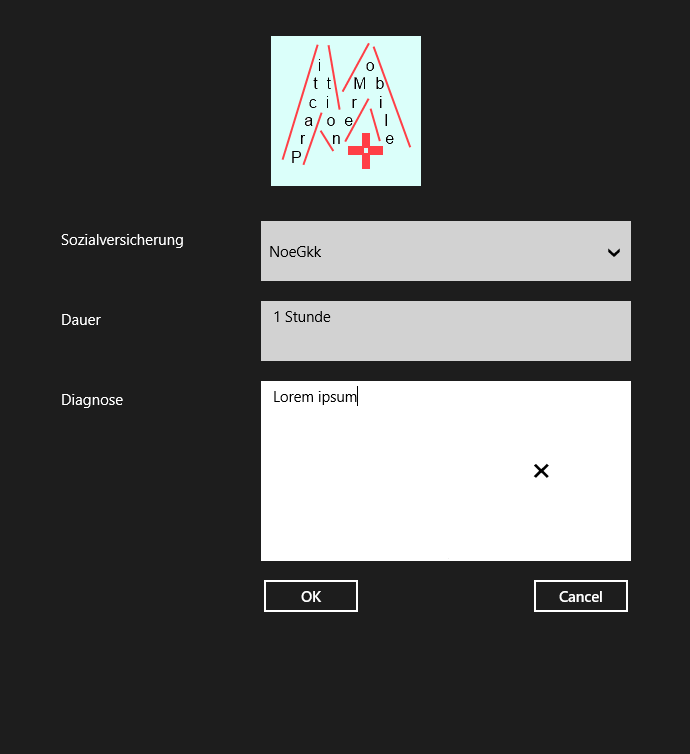
\includegraphics[scale=0.7]{images/customcontrol.png}
\caption[Custom Control]{Custom Control}\label{img:customcontrol}
\end{figure}
\newline
Neben den Dependency Properties werden auch zwei \textit{TappedEventHandler} deklariert, die für die Logik beim Betätigen des \textit{OK-} oder \textit{Cancel-}Buttons verantwortlich sind.
\newline
\newline
Das fertige Control kann man im \textit{ToolExplorer} von Visual Studio wiederfinden. Von dort muss es nur noch in ein XAML-File gezogen werden und ist anschließend vollständig einsatzbereit.

% http://stackoverflow.com/questions/15179188/cant-find-element-in-winrt-xaml
% Ok, it all seemed to work pretty well. Thanks! Last question though, what exactly does this do? [TemplatePart(Name = "_OK", % Type = typeof(Button))]
% I think it defines which elements are required in the template if someone changes the template of your control.
% wpf10 kap.17

%-------------------------------------------------------------------------------------------------------------------------------------------------------

\chapter[Schnittstellen und Charms]{Schnittstellen und Charms}\label{charms}
Neben den ursprünglichen, auf WinRT umgemappten API-Aufrufen gibt es auch ein Set von komplett neuen APIs. Viele davon sind in der Charm-Bar zusammengefasst, welche mit den neuen Windows-Versionen eingeführt wurde. Die Charm-Bar ist eine Art Menüleiste, die auf der rechten Seite des Bildschirms durch eine Wischgeste oder dadurch erscheint, dass man die Maus in die rechte obere Ecke des Bildschirms bewegt. Hier finden sich appspezifische Einstellungen und Funktionen. Die neuen Möglichkeiten, die Entwicklern dadurch offenstehen, werden in diesem Kapitel erläutert.
Auf Abbildung \ref{Abb7} ist diese neue Art der Menüleiste auf der rechten Seite der Online-Wörterbuchsapplikation \textit{LEO} erkennbar.
\newline
\begin{figure}[htbp]
\centering
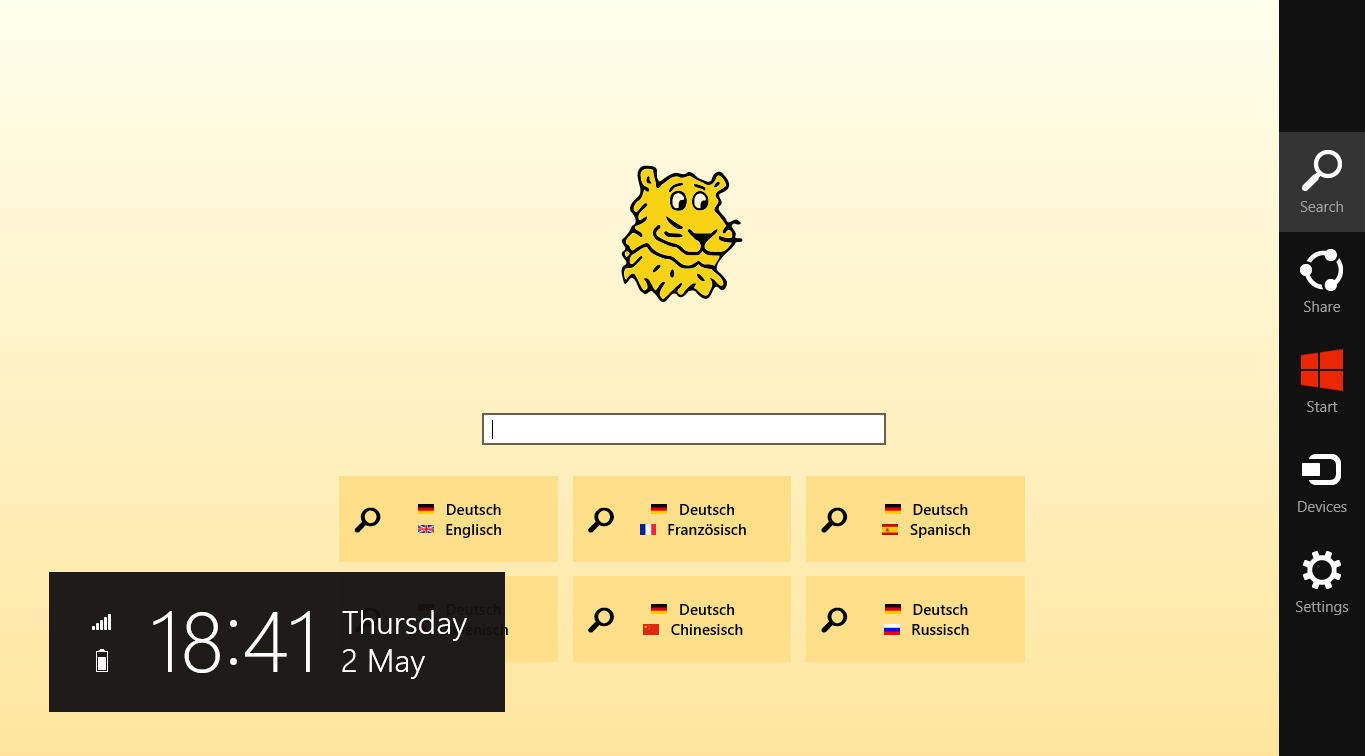
\includegraphics[scale=0.425]{images/charms.png}
\caption[Die neue Charms-Bart]{Die neue Charms-Bar}\label{Abb7}
\end{figure}
\newline

\section[Suchen]{Suchen}
Die Suche in WinRT Applikationen wurde im Vergleich zu den vorhergehenden Windows Versionen gründlich überarbeitet und mit neuen Funktionen ausgestattet. So ist es nun nicht mehr nur möglich, nach Dateien und Ordnern zu suchen. Zusätzlich kann man nun einen Suchbegriff eingeben, eine WinRT App auswählen und innerhalb einer App (welche diese Funktionalität explizit unterstützen muss) nach diesem Begriff suchen. So wird es unter anderem möglich, den Namen einer Stadt einzugeben, die Wetter-App auszuwählen, und direkt auf die Vorhersage an diesem Ort zuzugreifen. Wichtig dabei zu erwähnen ist, dass diese Applikation nicht laufen muss, nicht einmal im Hintergrund!
\newline
Die Suchresultate werden anschließend innerhalb der gewählten Applikation auf einer gesonderten Seite angezeigt, von wo aus man weitere Funktionen der Anwendung aufrufen kann.
\newline
\newline
Ein zusätzliches Feature der Suche ist das Anbieten von Suchvorschlägen beim Eintippen des Suchbegriffs. Auch die Logik hierhinter muss in der Applikation ausprogrammiert sein, kann dann aber eine weitere Usability-Verbesserung darstellen. Die Vorschläge werden ebenfalls in der Charms-Bar, direkt unter der Suchleiste angezeigt.
\cite {ana12}, S.477ff
\newline
\newline
Auch die später vorgestellte Applikation Practitioner Mobile verwendet die erwähnten Funktionalitäten. Demonstriert werden diese in Kapitel \ref{practmobile}.

\section[Teilen]{Teilen}\label{ref:share}
Die Teilen-Funktionalität ermöglicht es auf einfache Weise, Inhalte einer App mit anderen Applikationen zu teilen. Anstatt in etwa einen Text innerhalb einer Anwendung zu kopieren, das Mailprogramm zu öffnen, den Text dort einzufügen und anschließend zu versenden, könnte man dasselbe Resultat einfacher erzielen, indem man die Teilen-Funktion der Charm-Bar öffnet, ein Programm auswählt, das sich selbst als möglicher Empfänger klassifiziert (wie zum Beispiel das Mailprogramm), und direkt aus der gerade offenen Anwendung die Mail mit den gewünschten Inhalt verschickt.
\newline
\newline
Dieser ist dabei keinesfalls auf Text beschränkt, auch andere Objekte, von Bildern, spezielle Dokumente oder Binärdaten können geteilt werden. Wie der Inhalt dann weiter genutzt wird, entscheidet die App, die diesen entgegennimmt, programmatisch.
\newline
Zwei Properties, die beim Teilvorgang gesetzt werden, sind dabei besonders hervorzuheben: \textit{Title} und \textit{Description}. Diese werden in der Charm-Bar über der Liste der verfügbaren Apps angezeigt und entsprechen somit einer Art Vorschau, welche Daten geteilt werden. \cite {ana12}, S.486ff
\newline
Diese Funktion wird ebenfalls in Kapitel \ref{practmobile} demonstriert.

\section[Geräte]{Geräte}
Die Funktion \textit{Geräte} ist der \textit{Teilen} Funktionalität im Prinzip sehr ähnlich. Auch hier können Inhalte geteilt werden, diesmal allerdings nicht nur mit anderen Apps, sondern sogar mit anderen Geräten. Diese müssen allerdings Windows-zertifiziert sein, darunter fallen Geräte wie in etwa Drucker, Lautsprecher oder Ähnliches. Eine Quelle von so geteiltem Inhalt zu werden ist dagegen deutlich einfacher und mit ein wenig Code können Inhalte an einen Drucker, an Microsoft OneNote oder den Microsoft XPS Document Writer gesendet werden. \cite {ana12}, S.492ff
\newline
\newline
Wie einfach diese Art des Teilens ist, wird in Kapitel \ref{practmobile} gezeigt.

\section[Einstellungen]{Einstellungen}\label{einstellungen}
Wie auch die zuvor erwähnten Funktionen, sollen auch die Applikationseinstellungen an einem zentralen Punkt auffindbar sein. Der letzte Eintrag in der Charms-Bar ist genau dafür reserviert. Bis zu acht eigene Anpassungen lassen sich so zentral an einer Stelle durchführen.
\newline
\newline
Beim Klicken auf einen Link innerhalb dieses Einstellungs-Tabs kann im Prinzip jeder beliebige Code ausgeführt werden. Konvention ist es allerdings, im XAML einen neuen Bereich zu definieren, der dem Settings-Screen sehr ähnlich sieht und in welchem man genauere Anpassungen durchführen kann. Der Name des Controls, das für diesen Zweck häufig verwendet wird, ist \textit{Popup}. Dieses besitzt bereits von Haus aus Animationen und einen Zurück-Button, dessen Funktionalität man allerdings programmatisch selbst implementieren muss. \cite{ana12}, S. 503f
\newline
\newline
WinRT bietet außerdem noch eine zusätzliche Funktionalität an - Einstellungen können nun auch zwischen unterschiedlichen Geräten, auf denen der User mit derselben Live-ID angemeldet ist, synchronisiert werden. Microsoft nennt diese Funktion \textit{Roaming Settings}. Die Menge der Daten, die synchron gehalten werden können, ist allerdings sehr begrenzt - lediglich 100 Kilobytes werden derzeit von Microsoft erlaubt. Aus diesem Grund sollten nur wichtige Informationen geroamt werden, wie in etwa ein Spielstand, an welcher Stelle man die App verlassen hat, oder eben Einstellungen.
\newline
Außerdem gibt es keine Garantie dafür, dass die Einstellungen sofort nach Änderungen synchronisiert werden, so kann es durchaus durch Netzwerkprobleme zu Verzögerungen kommen, und außerdem kann der User das Roaming-Verhalten seines Gerätes auch komplett deaktivieren. In diesem Fall steht dem Entwickler die Roaming-Funktion nicht zur Verfügung und muss sich um eine andere Art der Persistierung kümmern.
\cite{ana12}, S. 463

\section[Lokale Daten und Datenbankanbindung]{Lokale Daten und Datenbankanbindung}
Da - wie im vorherigen Unterkapitel \ref{einstellungen} erwähnt - nur 100 Kilobyte geroamt werden dürfen, muss man sich als Entwickler eine andere Art der Datensicherung suchen, falls man mehr Informationen speichern will.
\newline
Eine Möglichkeit ist es, sogenannte \textit{App Files} anzulegen. Diese sind reguläre Files am normalen Filesystem, auf die andere WinRT Apps jedoch keinen Zugriff haben, da diese in einem speziellen abgetrennten Bereich abgelegt werden. Begrenzungen in der Größe der Dokumente gibt es lokal nicht, die Unterordner-Hierarchie darf lediglich eine Tiefe von 32 nicht überschreiten.
\newline
\newline
Datenbankanbindung an SQL Server wird derzeit nicht unterstützt - falls eine Datenbank benötigt wird, kann man aber auf File-basierte Datenbanken wie SQLite zurückgreifen.
\newline
\newline
Auch temporäre Dateien können bei Bedarf sehr einfach erstellt werden. Diese existieren selten länger als eine App-Session lang.
\cite{ana12}, S.464ff

% \section[File Picker Contract]{File Picker Contract}

\section[App Bars]{App Bars}
Die AppBars sind eine besondere Art von Control und bestehen aus Balken, die sich vom oberen oder unteren Rand der Applikation über die normale Views legen. Standardmäßig sind diese Balken ausgeblendet, durch einen rechten Mausklick oder eine entsprechende Geste werden sie erst ein-, beziehungsweise wieder ausgeblendet. Inhaltlich sollten diese Bars Buttons enthalten, die zusätzliche Optionen anbieten, sich aber nicht direkt auf der View befinden sollen, weil sie dort zu viel Platz einnehmen oder einfach nicht dorthin passen. Gruppiert werden können diese Buttons in den bereits in \ref{ref:panels} vorgestellten Panels.
\cite{ana12}, S.196ff

\section[Live Tiles]{Live Tiles}
Defaultmäßig wird eine App am Windows 8 oder Windows RT Startbildschirm mit seinem statischen Logo angezeigt. Neu ist allerdings die Unterstützung für sogenannte Live Tiles. Diese bieten einem die Möglichkeit, dynamisch ständig neue Informationen direkt am Startbildschirm anzuzeigen. Auch sekundäre Tiles können erstellt werden, die dem User einen Shortcut auf einen bestimmten Bereich einer App ermöglichen.
\newline
\newline
Wie ein Live Tile am Bildschim angezeigt wird, wird durch ein Template bestimmt, welches durch einen XML String definiert ist. Es können entweder auf verschiedene lokal gesicherte Informationen zurückgegriffen, oder aber in periodischen Abständen neue Daten aus dem Internet abgefragt werden. Wie Push Notifications dazu beitragen können, wird in \ref{pushnots} erklärt.
\newline
\newline
Über ein Live Tile können auch \textit{Badges} gelegt werden. Diese werden als Overlay dargestellt, die zusätzliche Informationen, wie in etwa die Anzahl der neu eingegangenen Emails bei einer Mailapp, darstellen kann. \cite{ana12}, S.539ff
\newline
\newline
In Abbildung \ref{img:livetile} sieht man das Live Tile der \textit{Bing Wetter} Applikation, die regelmäßig aktuelle Daten aus dem Internet abfragt.
\newline
\begin{figure}[htbp]
\centering

\includegraphics[scale=1.2]{images/livetile.png}
\caption[Live Tile]{Live Tile}\label{img:livetile}
\end{figure}

\section[Toast Notifications]{Toast Notifications}
Toast Notifications sind vergleichbar mit einer Message Box: sie erscheinen im rechten oberen Rand des Bildschirms und machen den User auf etwas Bestimmtes aufmerksam. Ignoriert dieser die Nachricht, verschwindet sie automatisch nach einer bestimmten Zeitspanne. 
\newline
Toast Notifications werden analog zu Live Tiles durch XML und Templates definiert, angezeigt werden sie entweder periodisch, oder programmatisch im Code. \cite{ana12}, S.552ff

\section[Push Notifications]{Push Notifications}\label{pushnots}
Um in periodischen Abständen aktuelle Informationen aus dem Internet abzufragen, oder um von seinen eigenen Servern Nachrichten an Benutzer einer Applikation senden zu können, kann man das Windows Push Notification Service (WNS) nutzen.
\begin{figure}[htbp]
\centering
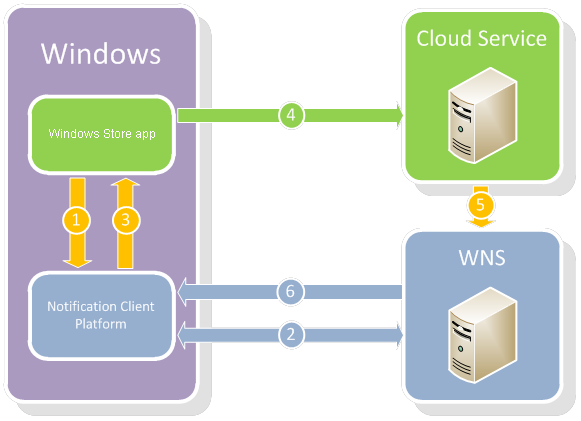
\includegraphics[scale=0.8]{images/push.png}
\caption[Nutzung des Push Notification Service]{Nutzung des Push Notification Service}\label{img:push}
\end{figure}
\newline
Dieses funktioniert, wie auch in Abbildung \ref{img:push} visualisiert wird, folgendermaßen:
\begin{itemize}
\item Die Applikation sendet eine Push Notification Request an die Notification Client Plattform und fragt um einen Kommunikationskanal an.
\item Die Notification Client Plattform leitet diese Anfrage an das WNS weiter, welches diesen im Erfolgsfall als Uniform Resource Identifier (URI) zurückliefert.
\item Diese URI wird jetzt wieder an die aufrufende WinRT App returniert. Sie kann an den eigenen Cloud-Dienst weitergeleitet werden und ab sofort als Kommunikationskanal zwischen Cloud Service und Applikation dienen.
\item Sobald der Cloud Service eine Update-Nachricht zur Verfügung hat, benachrichtig dieses den WNS über die erhaltene URI und eine HTTP POST Request. Dieses liefert die erhaltene Nachricht anschließend an das referenzierte Gerät aus.
\end{itemize}
Damit eine Applikation überhaupt Push Notifications empfangen kann, muss diese für diesen Dienst registriert sein. Die Authentifikation geschieht dann über das OAuth 2.0 Protokoll. \cite{push12}

\section[Sensoren]{Sensoren}
Tablets bieten Unterstützung für eine ganze Reihe von zusätzlicher Hardware an, die stationäre Geräte nicht besitzen und für die diese auch wenig sinnvoll wäre. Darunter können sich folgende Sensoren befinden: ein Beschleunigungsmesser, ein Gyrometer, ein Abweichungsmesser, ein Kompass, ein Lichtsensor, ein Orientierungssensor, ein Ortungssensor oder ein NFC-Chip. \cite{ana12}, S.529ff
\newline
Die Anzahl der Möglichkeiten ist also so groß wie noch nie. Es macht oftmals keinen Sinn, Unterstützung für alle der oben genannten Sensoren anzubieten, aber je nach Applikation sind diese zusätzlichen Optionen eine echte Bereicherung.

%-------------------------------------------------------------------------------------------------------------------------------------------------------

\chapter[Praktisches Beispiel anhand einer einfachen Line Of Business Applikation]{Praktisches Beispiel anhand einer einfachen Line Of Business Applikation}\label{practmobile}
In diesem Abschnitt werden die Highlights der für diese Bachelorarbeit entwickelten Applikation \textit{Practitioner Mobile} vorgestellt.
\newline
Practitioner Mobile ist ein Programm, dass es praktischen Ärzten ermöglichen soll, auch unterwegs Informationen über ihre Patienten und über Medikamente abrufen zu können. Die Anwendung ist simpel gehalten und mit nicht persistenten Testdaten befüllt. Ihr Zweck ist es nicht, tatsächlich einmal im Windows Store zu erscheinen, sondern dient rein zu Demonstrationszwecken.
\section[Charms]{Charms}
In diesem Abschnitt werden einige der bereits unter Kapitel \ref{charms} vorgestellten Möglichkeiten durch Charms in die Praxis umgesetzt.

\subsection{Suche}
Um einen Vertrag für die Suche zu erstellen, sind nur wenige Klicks notwendig. Der Großteil der Arbeit wird von Visual Studio selbst erledigt, selbst braucht man nur einen neuen \textit{Search Contract} über \textit{Add -> New Item -> Search Contract} erstellen und anschließend das neu erstellte File \textit{SearchResultsPage1.xaml.cs} mit eigener Suchlogik füllen. Außerdem muss eine neue sealed Klasse erstellt werden, die für die Suchresultate verwendet wird und mindestens folgende vier Properties besitzen muss:
\begin{itemize}
    \item public Uri Image
    \item public string Title
    \item public string Subtitle
    \item public string Description
\end{itemize}
Über die gefundenen Suchresultate kann anschließend zu einer anderen Seite innerhalb der Applikation navigiert werden, die zusätzliche Details über den Sucheintrag oder Ähnliches anzeigt.
\newline
Da Practitioner Mobile keinen persistenten Speicher implementiert, wird dieser Schritt übersprungen und auch nur statische Suchresultate zurückgegeben, anstatt die, welche einer echten Suche entsprechen würden.
\newline
\newline
Das UI der erstellten Suche für Pracitioner Mobile ist in Abbildung \ref{img:search} zu sehen.
\begin{figure}[htbp]
\centering
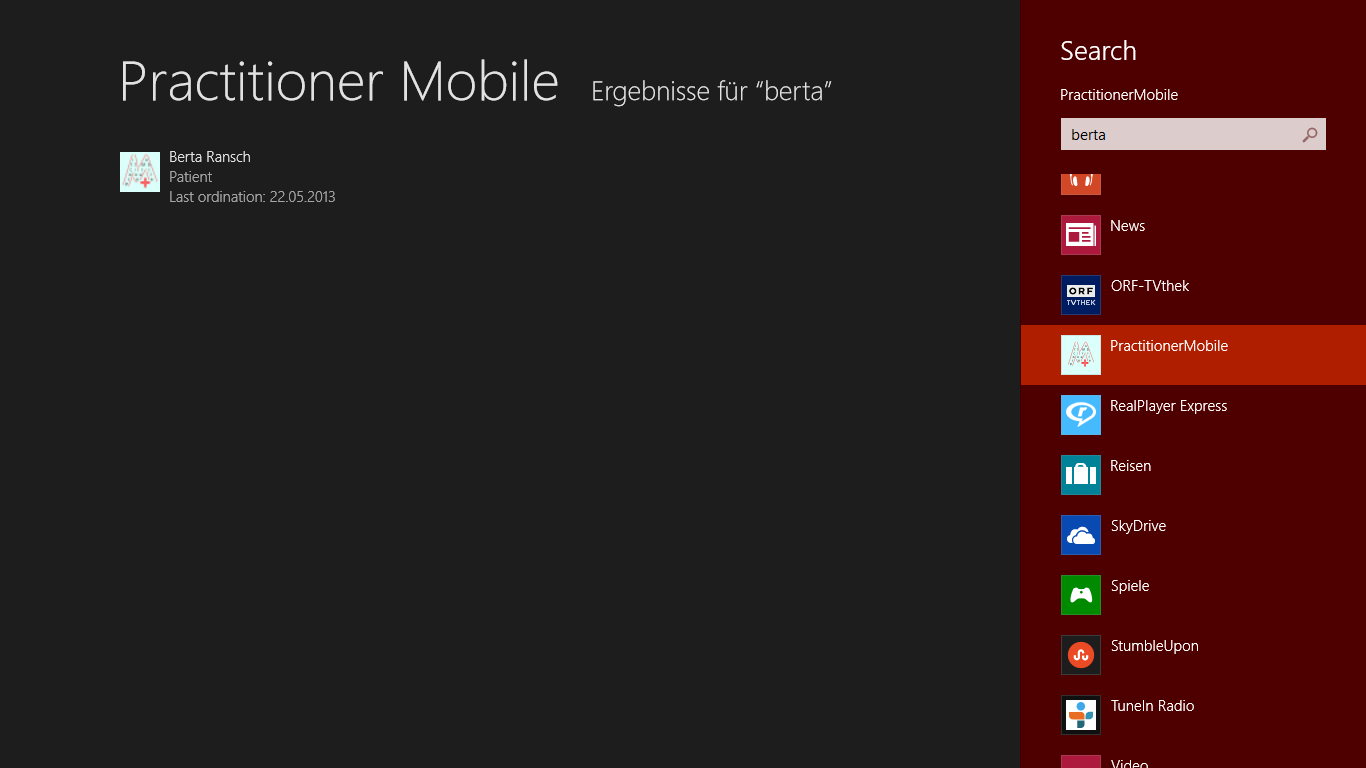
\includegraphics[scale=0.4]{images/search.png}
\caption[Suche]{Suche}\label{img:search}
\end{figure}
\newline
\subsection[Teilen]{Teilen}
Im Unterkapitel \ref{ref:share} wurde bereits erwähnt, welche Möglichkeiten es für eine Applikation gibt, um Inhalte zu teilen und anderen Applikationen zur Verfügung zu stellen.
\newline
Practitioner Mobile soll die Möglichkeit unterstützen, Daten eines Patienten an eine andere Applikation, wie einem Mailprogramm oder Microsofts OneNote, weiterzugeben.
\newline
Umgekehrt könnte auch unsere Applikation in etwa Patientendaten von einem anderen Programm empfangen und verarbeiten, dieser Schritt wird allerdings in Practitioner Mobile nicht demonstriert.
\newline
\newline
Daten zu teilen ist denkbar simpel. Es reicht aus, in der betreffenden View ein zusätzliches Event zu registrieren, das aufgerufen werden soll, wenn vom \textit{DataTransferManager} Daten angefragt werden:
\begin{lstlisting}[caption={Daten teilen}\label{lst:sharing},captionpos=t]
public MainPage()
{
[...]
DataTransferManager dataTransferManager = 
	DataTransferManager.GetForCurrentView();
 dataTransferManager.DataRequested += 
	OnDataRequested;
}
[...]
private void OnDataRequested
	(DataTransferManager sender, DataRequestedEventArgs args)
        {
            // Get selected patient
            Patient selectedPatient;
            try
            {
                selectedPatient = Patients
		.Where(p => p.Name == (this.ElementPanel.SelectedItem
				 as Patient).Name).FirstOrDefault();
            }
            catch(NullReferenceException)
            {
                // No patient selected - nothing to share
                return;
            }

            // Shown data in Share pane
            args.Request.Data.Properties.Title = selectedPatient.Name;
            args.Request.Data.Properties.Description 
		= "Last ordination: " + selectedPatient.LastOrdination;

            // Ordination data
            StringBuilder textToSet = new StringBuilder();
            textToSet.AppendLine("Ordinations:");

            foreach(Ordination o in selectedPatient.Ordinations)
            {
                textToSet.AppendLine( o.Date.ToString() + ", " +
		 o.SocialInsurance + ", " + o.DurationMinutes + 
		"Minutes, " + o.Diagnosis);
                textToSet.AppendLine("---");
            }

            args.Request.Data.SetText(textToSet.ToString());
        }
\end{lstlisting}
Wie das fertig aussieht, ist in Abbildung \ref{img:share} visualisert.
\begin{figure}[htbp]
\centering
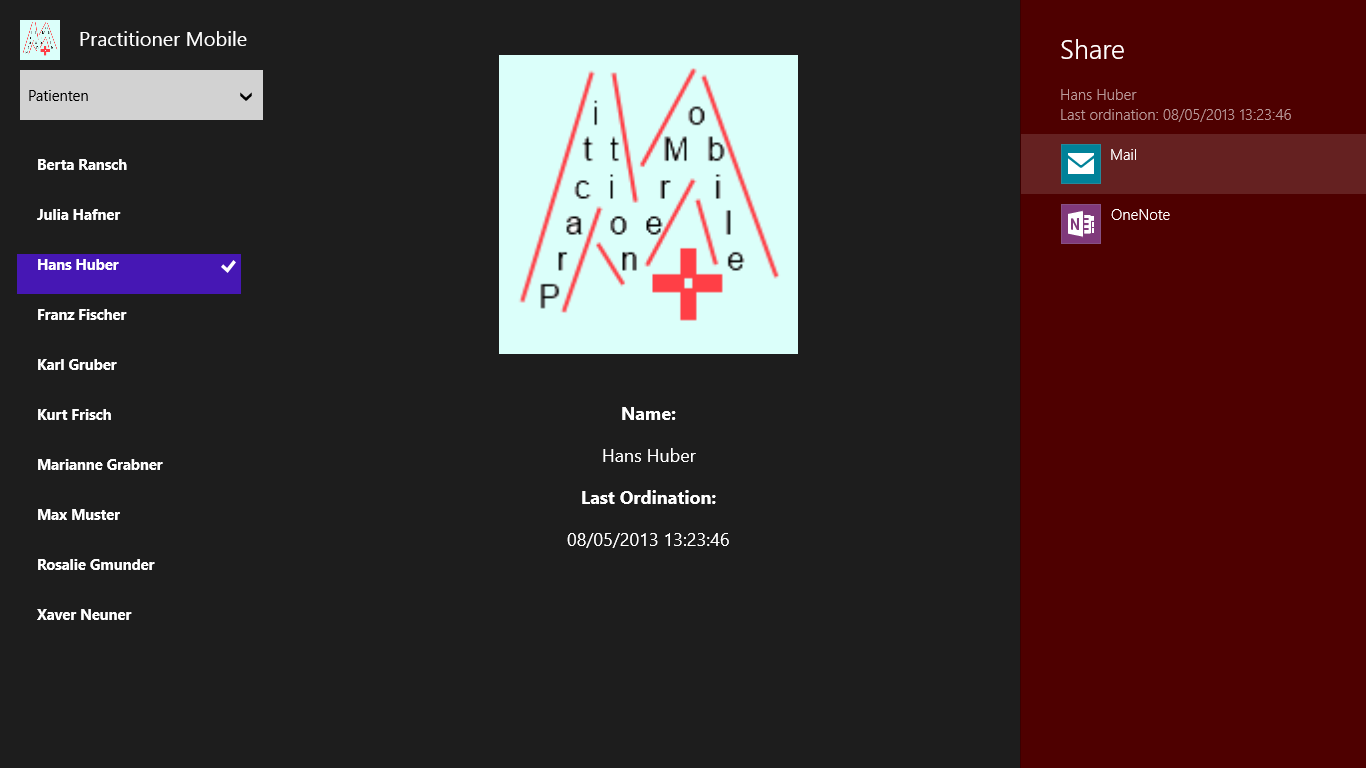
\includegraphics[scale=0.4]{images/share.png}
\caption[Daten teilen]{Daten teilen}\label{img:share}
\end{figure}

\subsection[Geräte]{Geräte}
Wenn die Daten nicht geteilt, sondern in etwa an einen Drucker gesendet werden sollen, kommt der Charm-Eintrag \textit{Geräte} ins Spiel. Auch die Verwendung dieser Funktionalität ist sehr trivial, das exakte Positionieren der Elemente kann allerdings einige Zeit in Anspruch nehmen.
\begin{figure}[htbp]
\centering
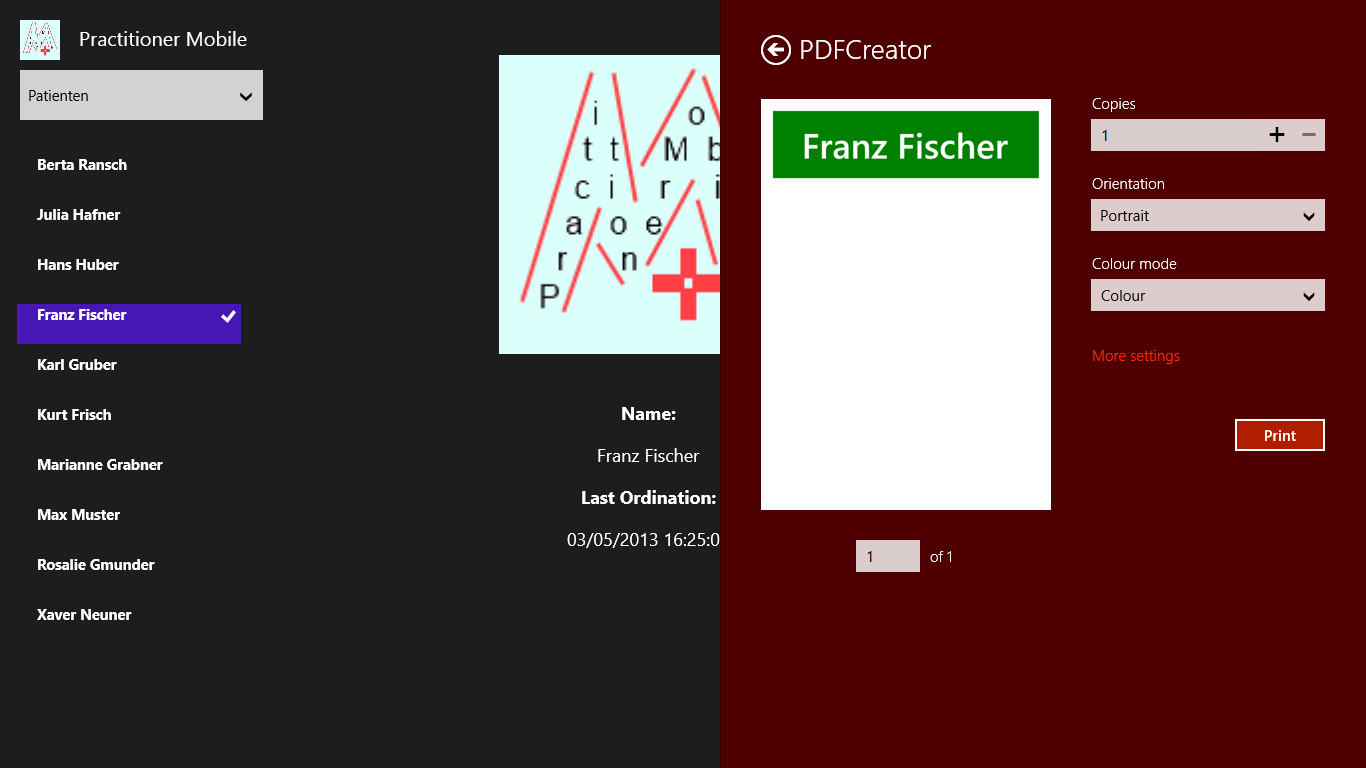
\includegraphics[scale=0.4]{images/print.png}
\caption[Daten drucken]{Daten drucken}\label{img:print}
\end{figure}
\newline
\newline
Der Einfachheit halber soll in Practitioner Mobile nicht mehr als der Name des Patienten gedruckt werden, grün hinterlegt, falls ein Patient ausgewählt ist, ein Hinweistext rot hinterlegt, falls das nicht der Fall ist. Angelehnt ist dieses Beispiel an das in \cite{ana12}, S. 493f.
\newline
\newline
Um die Druck-Funktionalität nutzen zu können, erzeugt man in der betroffenen View eine Instanz der Klasse \textit{PrintDocument} und sichert diese in einem lokalen Feld.
Anschließend registriert man eigene Eventhandler für die Events \textit{Paginate}, \textit{GetPreviewPage} und \textit{AddPages}.
\newline
Außerdem holt man sich die PrintManager-Instanz für die aktuelle View und hängt sich an das Event \textit{PrintTaskRequested} mit einer eigenen Methode an, wie in Listing \ref{lst:print} dargestellt.
\begin{lstlisting}[caption={Daten drucken}\label{lst:print},captionpos=t]
PrintDocument printDocument;

public MainPage()
{
     [...]
     this.printDocument = new PrintDocument();
     this.printDocument.Paginate += OnPaginate;
     this.printDocument.GetPreviewPage += OnGetPreviewPage;
     this.printDocument.AddPages += OnAddPages;
 
    PrintManager printManager = PrintManager.GetForCurrentView();
    printManager.PrintTaskRequested += OnPrintTaskRequested;
}
\end{lstlisting}
Die ausimplementierten Methoden sind in Appendix \ref{app:print} dargestellt.

\chapter[Fazit]{Fazit}
fazit
%-------------------------------------------------------------------------------------------------------------------------------------------------------

% Literaturverzeichnis
% Das Literaturverzeichnis kann auch nach einem allf"alligen Anhang positiioniert werden (siehe "`Leitfaden f"ur Bachelor- und Diplomarbeiten"', Version 2.0, Abschnitt 2.9).

% M"oglichkeit 1: Erzeugung des Literaturverzeichnisses mit BibTeX:
% Die Quellen sind in der Datei *.bib (hier Literatur.bib) einzugeben. Danach muss diese Vorlage einmal geTeXt werden, dann BibTeX angewendet werden und 
% anschliessend nochmals zweimal geTeXt werden.
% Im Text erfolgt die Zitierung mit dem Anker-Schl"usselwort, z.B. \cite{kop05}.
\bibliographystyle{IEEEtran}
\bibliography{Literatur}

% M"oglichkeit 2: Erzeugung eines Literaturverzeichnisses ohne BibTeX:
%\begin{thebibliography}{99}
%\bibitem[kop05]{kop05}
%H.~Kopka, {\em LaTeX, Band 1: Einf"uhrung}, Pearson Studium, M"unchen, 3.~Auflage, 2005.
%\bibitem[knu98]{knu98}
%F.~Mittelbach, M.~Goossens, J.~Braams, D.~Carlisle, and Ch. Rowley, {\em The LaTeX Companion}, 
%Addison-Wesley, 2nd edition, 2004.
%\end{thebibliography}

% Abbildungsverzeichnis
\listoffigures
\addcontentsline{toc}{chapter}{Abbildungsverzeichnis} % f"ugt den Eintrag "Abbildungsverzeichnis" im Inhaltsverzeichnis hinzu
\newpage

% Listingverzeichnis
 \lstlistoflistings
\addcontentsline{toc}{chapter}{Listingverzeichnis} % f"ugt den Eintrag "Listingverzeichnis" im Inhaltsverzeichnis hinzu
\newpage

% Tabellenverzeichnis
\listoftables 
\addcontentsline{toc}{chapter}{Tabellenverzeichnis} % f"ugt den Eintrag "Tabellenverzeichnis" im Inhaltsverzeichnis hinzu
\newpage

% Abk"urzungsverzeichnis
% Bei Verwendung der Dokumentklasse "scrartcl" ist der Befehlt \addchap{Abk"urzungsverzeichnis} durch 
% \addsec{Abk"urzungsverzeichnis} zu ersetzen
\addchap{Abk"urzungsverzeichnis}
\hspace{-17mm}\begin{tabular}{>{\raggedleft}p{0.2\linewidth} p{0.75\linewidth} p{0.1\linewidth}}
API & Application Programming Interface \\
CLR & Common Language Runtime \\
IDC & International Data Corporation \\
IMEA & Europa, Mittlerer Osten und Afrika \\
LOB & Line Of Business \\
PC & Personal Computer \\
UI & User Interface \\
URI & Uniform Resource Identifier \\
WinRT & Windows Runtime \\
WNS &  Windows Push Notification Service \\
WPF & Windows Presentation Foundation \\
XAML & Extensible Application Markup Language \\
XML & Extensible Markup Language
\end{tabular}

% Anh"ange
\begin{appendix}
\chapter[Custom Control]{Custom Control}\label{app:customcontrol}
\begin{lstlisting}[caption={Generic.xaml}\label{lst:Generic.xaml},captionpos=t]
<ResourceDictionary
 xmlns="http://schemas.microsoft.com/winfx/2006/xaml/presentation"
 xmlns:x="http://schemas.microsoft.com/winfx/2006/xaml"
 xmlns:pc="using:PractitionerMobile.Controls">

 <Style TargetType="pc:OrdinationMask">
     <Setter Property="Template">
         <Setter.Value>
             <ControlTemplate TargetType="pc:OrdinationMask">
                 <Border
                     Background="{TemplateBinding Background}"
                     BorderBrush="{TemplateBinding BorderBrush}"
                     BorderThickness=
			"{TemplateBinding BorderThickness}"
                     Width="600"
                     >
                     <Grid Name="OrdinationContentWrapper">
                         <Grid.ColumnDefinitions>
                             <ColumnDefinition Width="200" />
                             <ColumnDefinition Width="370" />
                         </Grid.ColumnDefinitions>
                         <Grid.RowDefinitions>
                             <RowDefinition Height="200" />
                             <RowDefinition Height="80" />
                             <RowDefinition Height="80" />
                             <RowDefinition Height="200" />
                             <RowDefinition Height="50" />
                         </Grid.RowDefinitions>
                         
                         <Image Grid.ColumnSpan="2" Grid.Row="0" 
			Grid.Column="0" 
			Source="{TemplateBinding ImagePath}" 
			Stretch="Uniform" Width="150" 
			Height="150" />
                         
                         <TextBlock Grid.Row="1" Grid.Column="0" 
			Text="Sozialversicherung" Margin="0,20,0,0"
			FontSize="15" />
                         <ComboBox Grid.Row="1" Grid.Column="1" 
			Name="SocialInsurance" 
			ItemsSource=
			"{TemplateBinding SocialInsurances}" 
			Height="60" />

                         <TextBlock Grid.Row="2" Grid.Column="0" 
			Margin="0,20,0,0" Text="Dauer" 
			FontSize="15" />
                         <TextBox Grid.Row="2" 
			Grid.Column="1" 
			Height="60" Name="Duration" />
                         
                         <TextBlock Grid.Row="3" Grid.Column="0" 
			Margin="0,20,0,0" Text="Diagnose" 
			FontSize="15" />
                         <TextBox Grid.Row="3" Grid.Column="1"
			 Height="180" Name="Diagnosis" />

                         <Button x:Name="Ok" Grid.Row="4" 
			Grid.Column="1" Content="OK"
			HorizontalAlignment="Left" 
			Width="100" Tag="ok" />
                         <Button x:Name="Cancel" Grid.Row="4" 
			Grid.Column="1" 
			Content="Cancel"
			HorizontalAlignment="Right" 
			Width="100" Tag="cancel" />
                     </Grid>
                 </Border>
             </ControlTemplate>
         </Setter.Value>
     </Setter>
 </Style>
</ResourceDictionary>
\end{lstlisting}

\begin{lstlisting}[caption={OrdinationMask.cs}\label{lst:OrdinationMask.cs},captionpos=t]
using System.Collections.Generic;
using Windows.UI.Xaml;
using Windows.UI.Xaml.Controls;
using Windows.UI.Xaml.Input;
using Windows.UI.Xaml.Media;

// The Templated Control item template is documented at 
// http://go.microsoft.com/fwlink/?LinkId=234235
namespace PractitionerMobile.Controls
{
    /// <summary>
    /// This class contains Practitioner Mobiles' custom control -
    /// a control, in which data of an ordination can be entered.
    /// </summary>
    [TemplatePart(Name = "Ok", Type = typeof(Button))]
    [TemplatePart(Name = "Cancel", Type = typeof(Button))]
    [TemplatePart(Name = "SocialInsurance", 
	Type = typeof(ComboBox))]
    [TemplatePart(Name = "Duration", Type = typeof(TextBox))]
    [TemplatePart(Name = "Diagnosis", Type = typeof(TextBox))]
    public sealed class OrdinationMask : Control
    {
        public OrdinationMask()
        {
            this.DefaultStyleKey = typeof(OrdinationMask);            
        }

     #region Public properties
     public string SocialInsurance
     {
	get;
	private set;
      }

    public int DurationMinutes
    {
	get;
	private set;
    }

    public string Diagnosis
    {
	get;
	private set;
    }
    #endregion

    #region Image
    public ImageSource ImagePath
    {
        get { return (ImageSource)GetValue(ImagePathProperty); }
        set { SetValue(ImagePathProperty, value); }
    }

    // Using a DependencyProperty as the backing store
    // for ImagePathProperty. This enables animation, styling, 
    // binding, etc...
    public static readonly DependencyProperty 
	ImagePathProperty = 
           	 DependencyProperty.Register("ImagePath",
			 typeof(ImageSource),
			 typeof(OrdinationMask), 
			new PropertyMetadata(null));
    #endregion

    #region Social Insurances
    private static List<string> _defaultSocialInsurances = 
	new List<string>() { "NoeGkk", "Wgkk", "BVA" };

    public static readonly DependencyProperty 
	SocialInsurancesProperty =
              DependencyProperty.Register("SocialInsurances",
              typeof(IEnumerable<string>),
              typeof(OrdinationMask),
              new PropertyMetadata(_defaultSocialInsurances));

    public IEnumerable<string> SocialInsurances
    {
        get { return (IEnumerable<string>) 
	GetValue(SocialInsurancesProperty); }
        set { SetValue(SocialInsurancesProperty, value); }
    }
    #endregion

    #region Button logic
    public event TappedEventHandler OnOkButtonHit;
    public event TappedEventHandler OnCancelButtonHit;
	
    /// <summary>
    /// Saves TextBox values to properties and calls 
    /// custom OK-event.
    /// </summary>
    private void okButton_Tapped(object sender, 
	TappedRoutedEventArgs e)
    {
	if(OkButtonHit != null)
	{
		var selectedListBoxItem = ((ComboBox)GetTemplateChild
			("SocialInsurance")).SelectedItem;
		if (selectedListBoxItem == null)
			return;

		this.SocialInsurance = selectedListBoxItem.ToString();
		this.Diagnosis = ((TextBox)GetTemplateChild
			("Diagnosis")).Text;

		string duration = ((TextBox)GetTemplateChild
			("DurationMinutes")).Text;
		int minutes;
		bool couldParse = int.TryParse(duration, out minutes);
		this.DurationMinutes = couldParse && 
			minutes >= 0 ? minutes : 0;

		OkButtonHit(this, null);
	}

	this.ClearFields();
    }

    /// <summary>
    /// Calls custom event and clears fields.
    /// </summary>
    /// <param name="sender"></param>
    /// <param name="e"></param>
    private void cancelButton_Tapped(object sender, 
	TappedRoutedEventArgs e)
    {
        if(OnCancelButtonHit != null)
        {
            OnCancelButtonHit(this, null);
        }

        this.ClearFields();
    }
    #endregion

    /// <summary>
    /// Sets events to buttons.
    /// </summary>
    protected override void OnApplyTemplate()
    {
    base.OnApplyTemplate();

    Button okButton = (Button)GetTemplateChild("Ok");
    Button cancelButton= (Button)GetTemplateChild("Cancel");

    okButton.Tapped += okButton_Tapped;
    cancelButton.Tapped += cancelButton_Tapped;
    }

    /// <summary>
    /// Clears all fields of the control.
    /// </summary>
    private void ClearFields()
    {
        ComboBox socialInsurance = 
	(ComboBox)GetTemplateChild("SocialInsurance");
        TextBox duration = (TextBox)GetTemplateChild("Duration");
        TextBox diagnosis = (TextBox)GetTemplateChild("Diagnosis");

        socialInsurance.SelectedIndex = -1;
        duration.Text = string.Empty;
        diagnosis.Text = string.Empty;
    }
  }
}
\end{lstlisting}

\chapter[Drucken]{Drucken}\label{app:print}
\begin{lstlisting}[caption={Ausschnitt aus MainPage.xaml.cs},captionpos=t]
#region Devices / Printing
/// <summary>
/// Sets preview pages.
/// </summary>
private void OnGetPreviewPage(object sender, 
	GetPreviewPageEventArgs e)
{
   this.printDocument.SetPreviewPageCount(1, 
	PreviewPageCountType.Final);

   Patient selectedPatient = this.GetSelectedPatient();
   if (selectedPatient == null)
   {
      this.printDocument.SetPreviewPage
	(1, new Viewbox { Child = new Button 
		{ Content = "Kein Patient ausgewaehlt",
		Background = new SolidColorBrush(Colors.Red) }});
   }
   else
   {
         this.printDocument.SetPreviewPage
		(1, new Viewbox { Child = new Button 
		{ Content = selectedPatient.Name, 
		Background =
		new SolidColorBrush(Colors.Green) } });
   }
}

/// <summary>
/// Sets actual pages.
/// </summary>
private void OnAddPages(object sender, AddPagesEventArgs e)
{
    Patient selectedPatient = this.GetSelectedPatient();
   if (selectedPatient == null)
   {
       this.printDocument.AddPage(new Viewbox 
		{ Child = new Button 
			{ Content = "Kein Patient ausgewaehlt", 
			Background =
			new SolidColorBrush(Colors.Red) }});
   }
    else 
    {
       this.printDocument.AddPage(new Viewbox 
	{ Child = new Button
		 { Content = selectedPatient.Name, 
		Background = 
		new SolidColorBrush(Colors.Green) }});
     }

     this.printDocument.AddPagesComplete();
}

/// <summary>
/// Does actual printing - performed, when device
/// entry in Charms bar is selected.
/// </summary>
private void OnPrintTaskRequested(PrintManager sender,
	PrintTaskRequestedEventArgs args)
{
     PrintTask printTask = args.Request
		.CreatePrintTask("Practitioner Mobile",
           	async (taskArgs) =>
           	{
               	var deferral = taskArgs.GetDeferral();
              	 await this.Dispatcher.RunAsync(Windows.UI.Core
			.CoreDispatcherPriority.Normal, () =>
                   	{
                    	   taskArgs.SetSource(printDocument
						.DocumentSource);
                     	  deferral.Complete();
                   	});
           });
}

private void OnPaginate(object sender, PaginateEventArgs e)
{
    this.printDocument.SetPreviewPageCount(1, 
	PreviewPageCountType.Intermediate);
}
#endregion
\end{lstlisting}

\end{appendix}
\end{document}